\setchapterpreamble[o]{%
\dictum[--- \textsc{Louis Pasteur}, \emph{französischer Chemiker und Mikrobiologe}]{\Gun Theorie ist die Mutter der Praxis.\Gob}}
\renewcommand{\chapterheadstartvskip}{\vspace*{2cm}}

\chapter{Theoretische Grundlagen}
\label{chap:theoretischegrundlagen}

Die folgenden Abschnitte dienen dazu, die grundlegende Zusammenhänge verschiedener Fachgebiete zu beschreiben, um dem weiteren Verlauf der Arbeit einfach folgen zu können.

 Dazu erfolgt zunächst eine allgemeine Einführung in die \textit{Theorie der Optimalsteuerung} und der darauf aufbauenden \textit{\acrlong{mpr}}, um die Rahmenbedingungen für die folgenden Kapitel zu definieren. 
 
Im darauffolgenden Abschnitt werden die \textit{Grundlagen zur Kommunikation über Bussysteme} ausführlich beschrieben. Sie umfassen elektrotechnische Grundlagen zur Datenübertragung und Vernetzung von technischen Systemen sowie Aspekte der Nachrichtentechnik und Informatik. Anschließend werden die Grundlagen mithilfe der \textit{Modbus Kommunikationstechnologie} in einen Anwendungskontext gebracht, damit sie in Kapitel \ref{chap:anlagendesign} bei der Installation der Anlage angewendet werden können.

Weiterhin erfolgt eine Beschreibung der \textit{thermodynamischen Grundlagen}, die bei der Beschreibung der Prozesse und Modellbildung in Kapitel \ref{chap:modellbildung} angewandt werden. 

Abschließend erfolgt eine allgemeine \textit{Einführung in die Solar- und Gebäudetechnik}, um den Einfluss der Solarstrahlung auf die Raumtemperatur in Abschnitt \ref{sub:modsonne} beschreiben zu können.

\section{Grundlagen zur Modellprädiktiven Regelung}
\label{sec:mpc}

Die \textit{\acrlong{mpr}} ist ein Teilgebiet der angewandten Mathematik, welche sich mit der Regelung von Prozessen oder technischen Systemen hinsichtlich gewählter Optimalitätskriterien beschäftigt. Hierzu bedient sie sich mathematischer Modelle des zu steuernden Prozesses sowie den \textit{Grundlagen der Optimalsteuerung}. Zur optimalen Regelung eines Prozesses werden wiederholt Optimalsteuerungsprobleme gelöst, wodurch sich besondere Anforderungen an das Modell ergeben \cite[S.~10]{di14}. Daher erfolgt zunächst eine kurze Einführung in die Optimalsteuerung, bevor die Modellprädiktive Regelung genauer beschrieben wird.

\subsection{Optimalsteuerung}

Die \textit{Optimalsteuerung} ist ebenfalls ein Teilgebiet der angewandten Mathematik und dient dazu, dynamische Systeme anhand von spezifizierten Optimalitätskriterien optimal zu steuern. Durch die Lösung eines Optimalsteuerungsproblems werden Steuersignale bestimmt, sodass die spezifizierten Leistungskriterien minimiert beziehungsweise maximiert werden und das Systeme eventuell vorgegebenen physikalischen und nutzerdefinierten Neben- sowie Randbedingungen genügt \cite[S.~3f.]{ki04}.
Die Prozesse dynamischer Systeme lassen sich durch \textit{Zustände} und \textit{Parameter} modellhaft beschreiben. Erstgenannte stellen die zu steuernden Größen dar und gemeinsam mit den Parametern beschreiben sie das \textit{Systemverhalten}. Das Modell kann wie zuvor erwähnt durch \textit{Rand- und Nebenbedingungen} beschränkt werden. Weiterhin können die Zustände von \textit{Steuergrößen} beeinflusst werden, welche frei wählbar oder vorgegeben sein können. Diese werden auch als \textit{Controls} bezeichnet und können durch Grenzen eingeschränkt werden. Sie stellen einen Freiheitsgrad des Systems dar. Des Weiteren wird das Leistungskriterium durch die \textit{Kostenfunktion} zum Ausdruck gebracht. Das Optimalsteuerungsproblem lässt sich dann wie folgt beschreiben \cite[S.~61]{di14}:

\begin{eqnarray}
\label{eq:opt}
		{\text{minimize} \atop \vec{x}(.),\vec{u}(.)} & &\int_0^T L(\vec{x}(t),\vec{u}(t)) dt + E(\vec{x}(T)) \quad ,t \in [0,T] \\
\nonumber		&&\\
\nonumber		\text{subject}\; \text{to} & &\\
\nonumber		\vec{x}(0)-\vec{x}_{0} & = & 0,	\qquad \text{(Fixed Initial Value)}\\
\nonumber		\stackrel{.}{\vec{x}}-f(\vec{x}(t),\vec{u}(t)) & = & 0,\qquad \text{(ODE Model)}\\
\nonumber		h(\vec{x}(t),\vec{u}(t)) & \leq & 0, \qquad \text{(Path Constraints)}\\
\nonumber		r(\vec{x}(T)) & \leq & 0,\qquad \text{(Terminal Constraints).}
\end{eqnarray}

Die Zustände werden vom Zustandsvektor $\vec{x}$ und die Controls vom Vektor $\vec{u}$ beschrieben. Die Parameter sind implizit im Modell enthalten, welches durch ein Gleichungssystem aus gewöhnlichen Differenzialgleichungen (ODE Model) beschrieben wird. Die Kostenfunktion wird auch als \textit{Bolza Ziel} bezeichnet und besteht aus dem \textit{Lagrange-} und den \textit{Mayer-Term}. Letzterer beschreibt die Kosten zum Endzeitpunkt $T$ des Optimierungsintervalls wohingegen der Lagrange-Term den integralen Kostenanteil umfasst. Die Randbedingungen werden von den Initialwerten $\vec{x}(0)-\vec{x}_{0} = 0$ (Fixed Initial Value) und den Endbedingungen $r(\vec{x}(T)) \leq 0$ (Terminal Constraints) berücksichtigt. Die physikalischen und nutzerdefinierten Nebenbedingungen sind durch die Path Constraints $h(\vec{x}(t),\vec{u}(t)) \leq 0$ beschrieben. Anschaulich sind diese Zusammenhänge in \ref{fig:opt} dargestellt.

\begin{figure}
\centering
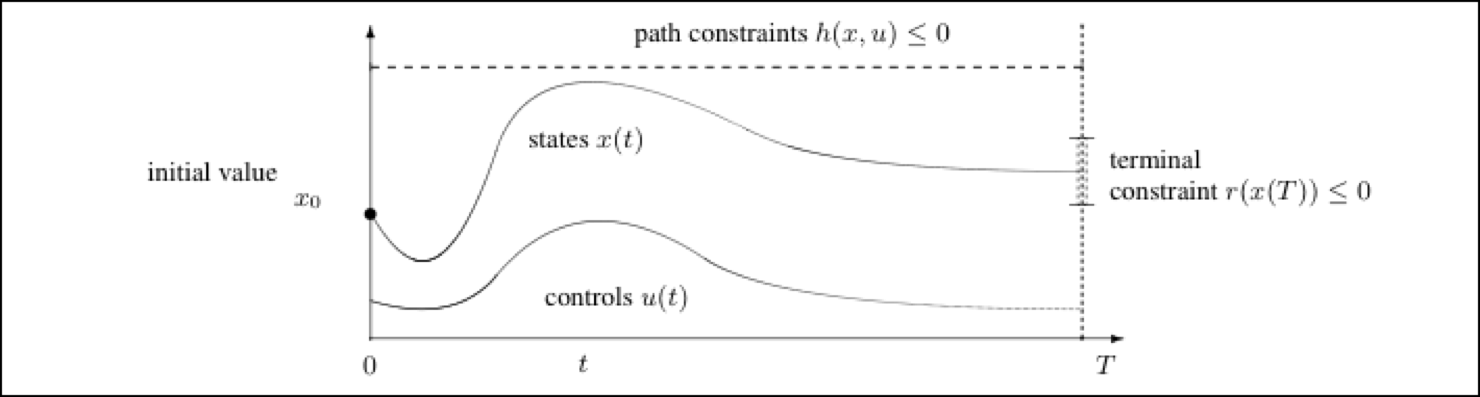
\includegraphics[width=\textwidth]{abbildungen/20160327_mpc}
\caption[Variablen, Neben- und Randbedingungen eines optimalen Steuerungsproblems]{Variablen, Neben- und Randbedingungen eines optimalen Steuerungsproblems, entnommen aus \cite[S.61]{di14}}
\label{fig:opt}
\end{figure}

Um eine \textit{optimale Lösung} dieses zeitkontinuierlichen Optimierungsproblems zu bestimmen, muss die erste Ableitung die \textit{notwendigen} \textit{Karush-Kuhn-Tucker} Bedingungen erfüllen. Weiterhin muss die zweite Ableitung einer \textit{hinreichenden} Bedingung genügen. Daher ist es notwendig, dass das nichtlineare Optimalsteuerungsproblem zweifach stetig differenzierbar ist und damit auch das mathematische Modell des Prozesses \cite[S.~21ff.]{di14}.

Eine \textit{optimale Lösung} beschreibt einen optimalen Einsatz von Steuergrößen -- hinsichtlich der formulierten Kostenfunktion -- zur Beeinflussung des Systems und wird auch als \textit{Optimalsteuerungsplan} bezeichnet.

Konkret können mehrere, numerische Ansätze zur Lösung des Optimalsteuerungsproblems verfolgt werden, die sich in den \textit{Zustandsraum}, die \textit{indirekten} sowie \textit{direkten Verfahren} einteilen lassen. Reale Probleme zeichnen sich durch eine Vielzahl an Nebenbedingungen aus. Diese eigenen sich besonders zur Optimierung mit direkten Verfahren, weshalb sie in der Praxis am weitesten verbreitet sind \cite[S.~63]{di14}. 
Da die \acrlong{mpr} nur den Rahmen dieser Arbeit bildet, wird nicht näher auf die Optimalsteuerung eingegangen. Der interessierte Leser findet in \cite{di14} eine theoretische fundierte Einführung zur Optimalsteuerung sowie eine ausführliche Beschreibung der einzelnen Lösungsverfahren.


\subsection{Modellprädiktive Regelung}

Da zwischen Modellen und den realen Prozessen immer Diskrepanzen bestehen, wird der Prozess durch den Einsatz eines berechneten Optimalsteuerungsplans mit höchster Wahrscheinlichkeit nicht exakt dem vorausberechneten Weg folgen. Dieses Phänomen wird auch als \textit{Model-Plant-Mismatch} bezeichnet. Die \acrlong{mpr} eignet sich hervorragend, um diesen Model-Plant-Mismatch sowie Störungen des Prozesses auszugleichen, ohne den Einsatz einer umfassenden \textit{Echtzeitregelung}. Eine solche Echtzeitregelung lässt sich aufgrund des enormen Rechenaufwands ohnehin nur durch Näherungen und Vereinfachungen für sehr einfache Anwendungen umsetzen. Diese Lücke wird durch die \acrlong{mpr} geschlossen. Sie betrachtet ein beschränktes, immer gleich weit in die Zukunft hinein ragendes Zeitintervall und versucht zu diskret wiederholten Zeitpunkten das Verhalten des Systems vorherzusagen. Dies geschieht durch eine Vorausberechnung mithilfe eines mathematischen Modells des Prozesses, aufbauend auf der Kenntnis des aktuellen Zustandes. Dabei wird gleichzeitig durch die periodisch Berechnung von Optimalsteuerungsplänen versucht, die projizierten Zustände dem gewählten Optimalitätskriterium entsprechend zu beeinflussen. Dadurch kann auf Abweichungen des Prozesses zum ursprünglichen Optimalsteuerungsplan zu diskreten Zeitpunkten reagiert, unabhängig davon ob diese durch eine Modellabweichungen oder Störungen bedingt sind \cite[S.~71]{di14}.

Im Rahmen dieser Arbeit wird eine Anlage aufgebaut und ein Modell gebildet, die eine Modellprädiktive Raumtemperaturregelung während des laufenden Betriebs ermöglichen sollen. 
Die hieraus abgeleiteten Anforderungen an eine Anlage werden im Kapitel \ref{chap:anlagendesign} bei der Anforderungsanalyse beschrieben.
Aus dieser Theorie ergeben sich weitere Anforderungen, welche bei der Modellbildung in Kapitel \ref{chap:modellbildung} dargelegt werden.


\section{Technische Grundlagen zur Kommunikation mit Bussystemen}
\label{sec:grundlagenbus}

In diesem Abschnitt werden die technischen Grundlagen von Hard- und Software beleuchtet, die zur Kommunikation technischer Systeme benötigt werden. Die Kommunikation findet zumeist über Bussysteme statt, deren Grundlagen zuerst erklärt werden. Anschließend wird das allgemeine \acrlong{osi} (\acrshort{osi}) zur Kommunikation beschrieben. Abschließend werden die zuvor erläuterten Grundlagen anhand der \textit{Modbus Kommunikationstechnologie} in einen Anwendungsbezug gesetzt.

\subsection{Bussysteme}

Um ganz allgemein Prozesse zu überwachen, zu steuern oder regeln zu können, müssen zwischen Prozessbeteiligten Informationen ausgetauscht werden. 
Die Prozessbeteiligten können technische Bauteile, Aktoren oder Sensoren sowie Controller sein, die zusammen ein technisches System bilden, welches im Folgenden als Anlage bezeichnet wird. Eine Anlage ist eine eigenständige funktionale Einheit, welche einen eigenen Zweck verfolgt. Sie zeichnet sich durch einen Mehrwert gegenüber der Summe der einzelnen Komponenten aus, der durch ein Zusammenspiel der Komponenten erreicht wird. Diese Emergenz wird durch die Kommunikation realisiert und ermöglicht der Anlage ihren Zweck zu erreichen.
Es zeichnet sich allerdings ein Trend hin zur drahtlosen Kommunikation ab, die jedoch noch stark vom Einsatzort und der Störanfälligkeit begrenzt wird. Im Kontext von technischen Systemen erfolgt die Kommunikation zumeist über Bussysteme, da sie eine hohe Robustheit gegenüber Störungen besitzen und auch in unfreundlichen Umgebungen eingesetzt werden können. Sie lassen sich anhand von verschiedenen Merkmalen klassifizieren. Im Folgenden werden die wichtigsten Merkmale beschrieben in Anlehnung an die Struktur von \cite{schn06}.


\subsubsection{Informationsaustausch}

Die \textit{Informationen} über einen Prozess und dessen Zustand werden auf hoher Ebene durch \textit{Daten} repräsentiert. Auf der untersten Ebene wird eine Information durch mehrere \textit{Bits} repräsentiert. Der Austausch von Daten findet in Form von \textit{Telegrammen} statt. Ein Telegramm besteht grundsätzlich aus zwei Teilen, den zu übertragenden Daten und den Informationen zur Übertragung. Die Daten werden vor der Übertragung in \textit{Rahmen}, sogenannte \textit{Data Frames}, eingeteilt. Der detaillierte Aufbau eines Telegramms wird vom eingesetzten Kommunikationsprotokoll innerhalb des Netzwerks definiert \cite[S.~11f.]{schn06}.

Im Detail wird die Struktur eines Telegramms in Abschnitt \ref{sub:modbus} am Beispiel von zwei Modbus Kommunikationsprotokollen erläutert. Eine graphische Illustration dazu findet sich in \ref{fig:modbusframe}.

\subsubsection{Netzwerk und Topologie}

Einzelne Komponenten der Anlage werden zur Kommunikation miteinander über \textit{Verbindungsleitungen} miteinander verbunden, welche zur Übertragung von Telegrammen genutzt werden. Dabei entstehen \textit{Netzwerke}, wobei die Komponenten der Anlage auch \textit{Netzwerkteilnehmer} bezeichnet werden. Ein Netzwerk lässt sich in einzelne Segmente einteilen und kann je nach Ausführung der Verbindungsleitungen und Anzahl der Teilnehmer unterschiedlich ausgeprägt sein. Anhand der geometrischen Anordnung lassen sich die folgenden, verschiedenen \textit{Netzwerktopologien} unterscheiden.


Die einfachste Art zwei Teilnehmer eines Netzwerks miteinander zu verbinden ist die sogenannte \textit{Zweipunktverbindung}. Dazu werden die Netzwerkteilnehmer jeweils durch eine direkte Leitung miteinander verbunden. Mit der Anzahl von Teilnehmern steigt jedoch auch der Verbindungsaufwand überproportional an, um in solch \textit{vermaschten Netzwerken} alle Teilnehmer miteinander zu verbinden. Dies hat für große vermaschte Netzwerke zur Folge, dass eine unübersichtlich große Anzahl von Schnittstellen und ein extrem hoher Verkabelungsaufwand entsteht, der wiederum mit hohen Kosten verbunden ist. Um diese Kosten zu vermeiden, ergeben sich noch weitere Möglichkeiten zur Verbindung und Anordnung von Netzwerkteilnehmern \cite[S.~1f.]{schn06}.


Um dem hohen Verkabelungsaufwand zu entgehen, wird bei großen Netzwerken zu einer \textit{Linienstruktur} übergegangen. Diese wird auch als \textit{Bus-Struktur} bezeichnet und ist in \ref{fig:bus_struktur} veranschaulicht. Charakteristisch für die Bus-Struktur ist, dass alle Teilnehmer entlang einer langen Verbindungsleitung, dem sogenannten \textit{Buskabel}, angeordnet sind. Sie sind mithilfe von kurzen \textit{Stichleitungen} an das gemeinsame Buskabel angebunden, über das die gesamte Kommunikation im Netzwerk erfolgt.

Durch diese Netzwerktopologie wird der Verkabelungsaufwand sowie die Anzahl an Schnittstellen stark reduziert, insbesondere für sehr große Netzwerke. Jedoch wird durch die Nutzung einer gemeinsamen Kommunikationsleitung eine gleichzeitige Kommunikation von mehreren Teilnehmern erschwert. Daher wurden sogenannte \textit{Buszugriffsverfahren} eingeführt, welche Zugriffsregeln auf die Busleitung definieren und im nachfolgenden Abschnitt beschrieben werden. Weiterhin müssen aufgrund der Parallelschaltung alle Teilnehmer ständig alle Telegramme mitverfolgen, wodurch der Sender stark belastet wird. 

Die Busleitungslängen sind außerdem meist sehr lange\footnote{Diese reichen von mehreren hundert Metern bis teilweise in den Kilometerbereich, je nach Art und Einsatzort der Anwendung.}. Daher ist die Länge der Leitung, bezogen auf die zu übertragende Wellenlänge, nicht mehr vernachlässigbar klein und die Busleitung muss zur Vermeidung von Reflexionen durch Leitungsabschlusswiderstände an beiden Enden abgeschlossen werden. Außerdem werden die Leitungslängen und die Teilnehmer je Netzwerksegment begrenzt \cite[S.~3f.]{schn06}.

\begin{figure}
\centering
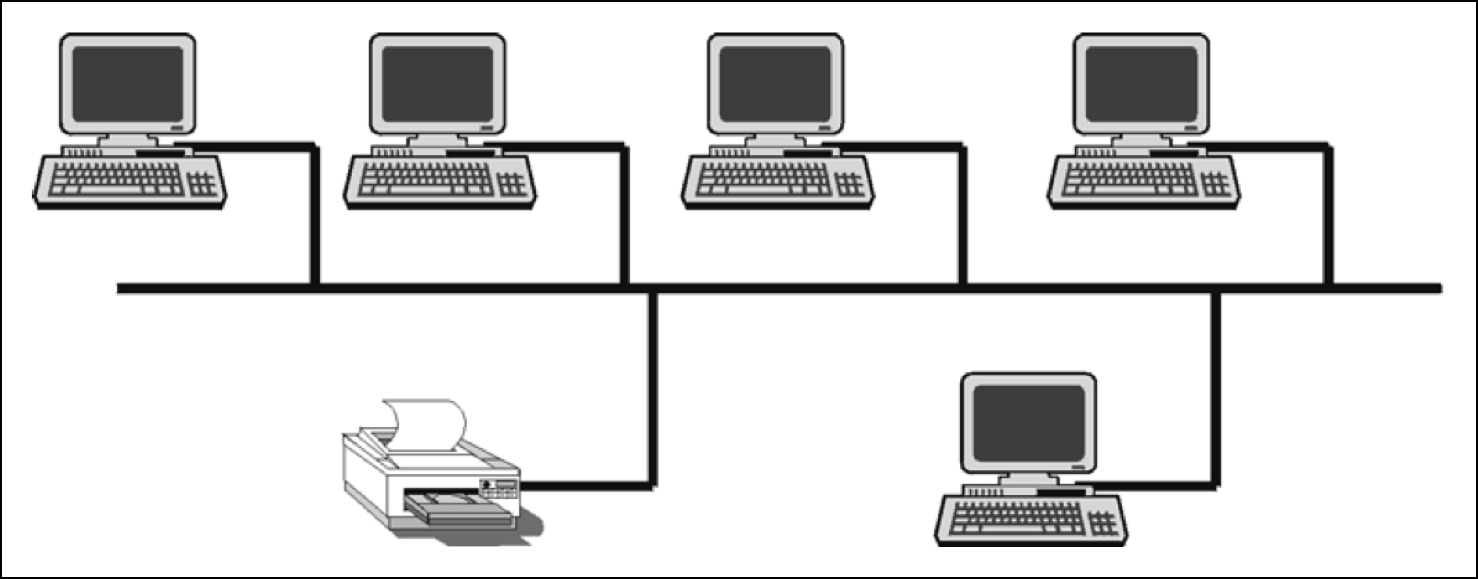
\includegraphics[width=\textwidth]{abbildungen/20160109_busstruktur}
\caption[Bus-Struktur]{Bus-Struktur,entnommen aus \cite[S.~3]{schn06}}
\label{fig:bus_struktur}
\end{figure}


Der Leitungs- und Kapazitätswiderstand einer Busleitung hängen unmittelbar von ihrer Länge ab und lassen sich durch das Ersatzschaltbild eines RC-Gliedes repräsentieren, wie in Abbildung \ref{fig:bus_impuls} a) zu sehen ist. Durch die beiden Widerstände entsteht eine Impulsverzerrung \gls{timp}, die somit mittelbar von der Leitungslänge abhängt.

Je länger die Leitung wird, desto größer werden auch die beiden Widerstände. Die Ladezeit steigt durch die erhöhte Leitungskapazität $C_{Leitung}$, gleichzeitig sinkt die Lastspannung $U_{G}$ durch den vergrößerten Leitungswiderstand $R_{Leitung}$. Dadurch verstärkt sich die Impulsverzerrung \gls{timp}, wie in \ref{fig:bus_impuls} b) und \ref{fig:bus_impuls} c) dargestellt.

Die maximale Frequenz \gls{fmax} der Datenübertragung wird auf den Kehrwert der Impulsverzerrung $f_{max}=\frac{1}{\Delta t_{Imp}}$ beschränkt, sodass der Empfänger den Wechsel des logischen Zustandes weiterhin registrieren kann. In der Praxis bedeutet dies, dass die Leitungslänge und die Übertragungsrate miteinander verknüpft sind und sich gegenseitig beeinträchtigen \cite[S.~4f.]{schn06}.

\begin{figure}
\centering
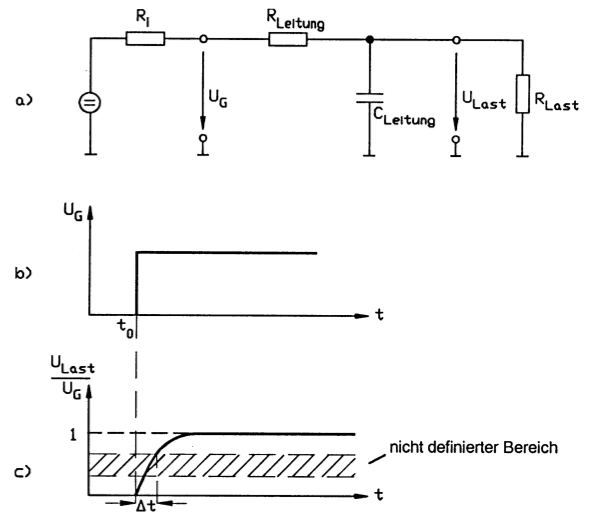
\includegraphics[width=\textwidth]{abbildungen/20160110_impulsbus}
\caption[Impulsverzerrung auf einer Leitung]{Impulsverzerrung auf einer Leitung: a) Ersatzschaltbild der Anordnung b) Ausgangsspannung des Generators c) Empfängerspannung, entnommen aus \cite[S.~4]{schn06}}
\label{fig:bus_impuls}
\end{figure}

Um die Beschränkung der Leitungslänge aufzulockern, wird die Bus-Struktur zu einer \textit{Baum-Struktur} weiterentwickelt.
In \ref{fig:baum_struktur} ist zu erkennen, dass mehrere Netzwerk-Segmente durch \textit{Verstärkerelemente} zu einem großen Netzwerk verknüpft werden. Die verschiedenen Segmente wiederum bestehen aus einzelnen Bus-Strukturen.
Es wird eine galvanische Trennung der Teilnehmer benötigt, um große Flächen zu vernetzen und und damit die Einschränkungen der Bus-Struktur zu umgehen \cite[S.5~f.]{schn06}.
Die Besonderheit dieser Struktur liegt darin, dass sie durch ihren Aufbau nachträgliche Erweiterungen mühelos ermöglicht. Die verschiedenen Bauteile zur Erweiterung eines Netzwerkes werden im nachfolgenden Abschnitt \ref{sub:schnitt} vorgestellt.

\begin{figure}
\centering
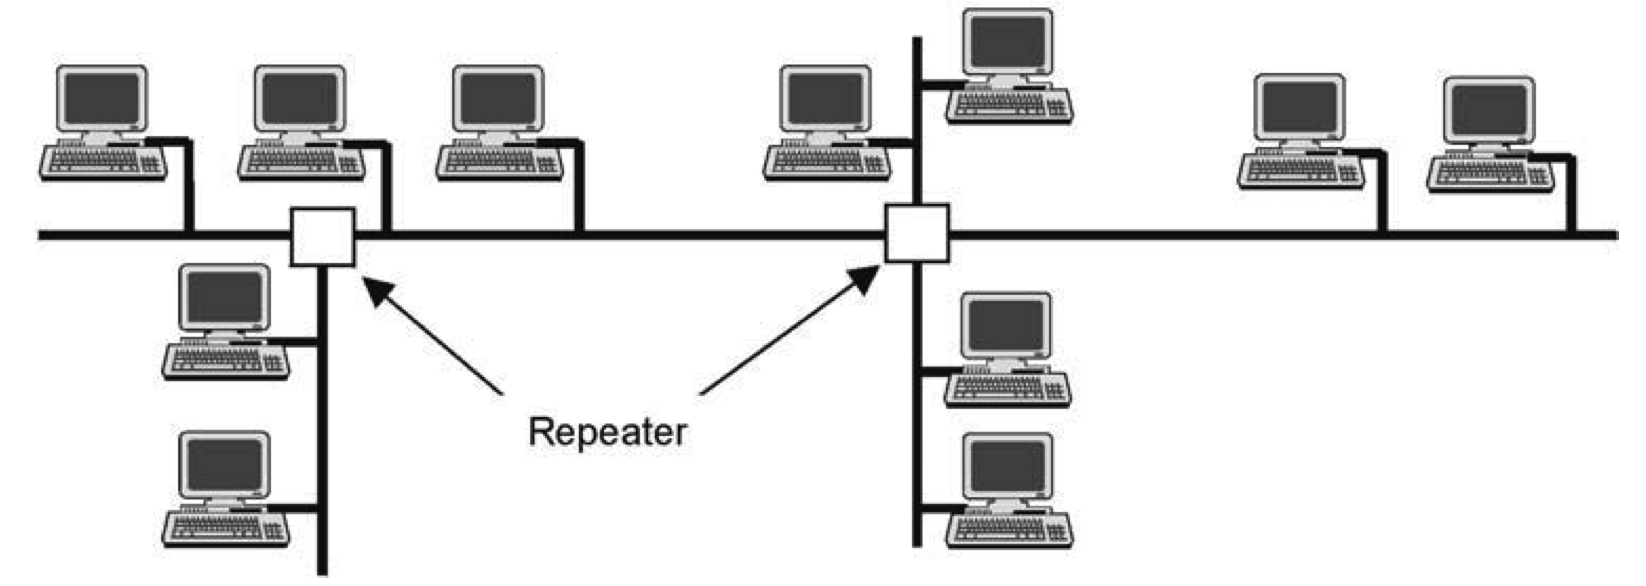
\includegraphics[width=\textwidth]{abbildungen/20160110_baumstruktur}
\caption[Baumstruktur]{Baumstruktur, entnommen aus \cite[S.~5]{schn06}}
\label{fig:baum_struktur}
\end{figure}

Weitere bedeutende Netzwerktopologien sind die \textit{Ring-} und die \textit{Stern-Struktur}, die für das Verständnis dieser Arbeit keine weitere Relevanz besitzen.
Die Ring-Struktur besteht aus einem physikalischen Ring von Zweipunktverbindungen und ist durch eine Kommunikation der Teilnehmer übereinander hinweg gekennzeichnet.
Bei der Stern-Topologie hingegen, sind die Netzwerkteilnehmer um eine Zentralstation herum angeordnet. Die gesamte Kommunikation läuft über die zentrale Komponente, die mit jedem einzelnen Teilnehmer verbunden ist. Der interessierte Leser wird für detaillierte Beschreibungen auf \cite{schn06} verwiesen.

\subsubsection{Buszugriffsverfahren}

Bei den meisten Netzwerktopologien erfolgt die Kommunikation  über eine gemeinsame Verbindungsleitung. Daher müssen Regeln für den Zugriff definiert werden, die eine reibungslose Kommunikation gewährleisten. \textit{Buszugriffsverfahren} lassen sich in zwei Gruppen untergliedern: in \textit{kontrollierte} und \textit{zufällige Verfahren} \cite[S.~19]{schn06}.

Bei den kontrollierten Verfahren ist der Sender bereits vor Sendebeginn eindeutig bestimmt, daher ist eine Zuteilung des Busses ist nicht erforderlich. Der Zugriff findet entweder zentral statt, bei den sogenannten \textit{Master/Slave-Verfahren}, oder wird dezentral durch Steuereinheiten geregelt, wie beispielsweise bei dem \textit{Tokenring} und \textit{Tokenbus}. Ein solches Verfahren heißt \textit{echtzeitfähig}, falls die Zykluszeit der Datenübertragung durch eine Beschränkung der maximalen Telegrammlänge und damit des Übertragungsintervalls bestimmbar ist.
Bei zufälligen Buszugriffsverfahren greifen die Teilnehmer bei Bedarf auf die Verbindungsleitung zu. Dabei müssen sie sicherstellen, dass die Busleitung nicht gleichzeitig von einem anderen Teilnehmer belegt ist. Es kann nicht bestimmt werden zu welchen Zeitpunkten Telegramme übertragen werden, wodurch keine Echtzeitfähigkeit vorliegt \cite[S.~19]{schn06}.

Beim Master/Slave-Verfahren kommen eine \textit{Bussteuerungseinheit}, der sogenannte \textit{Master}, sowie mehrere \textit{passive Teilnehmer}, die sogenannten \textit{Slaves}, zum Einsatz.
Die Kommunikation wird ausschließlich vom Master initiiert, indem er aktiv eine Verbindung zu den Slaves herstellt und \textit{Requests} sendet, in welchen die angeforderten Daten spezifiziert sind.
Die Slaves werden lediglich durch Anfragen aktiv und antworten unmittelbar mit einer \textit{Response}, welche die angeforderten Daten enthält.
Damit der Master ein umfassendes und aktuelles Bild über den Systemzustand bekommt, erfolgt die Kommunikation in der Regel in periodischen Intervallen zeitgleich mit allen Slaves (\textit{Polling}). Als Slaves können einfache und günstige Bauteile eingesetzt werden, da im Master die benötigte \Gun Intelligenz\Gob implementiert ist. 
Es gilt bei diesem Verfahren zu beachten, dass der Informationsaustausch zwischen verschiedenen Slaves längere Zeit in Anspruch nehmen kann und dass ein Ausfall des Masters das gesamte Bussystem stilllegt \cite[S.~19ff.]{schn06}.

Auf eine Beschreibung der übrigen Verfahren wird aufgrund der fehlenden Relevanz für diese Arbeit verzichtet. Weitere Ausführungen finden sich bei \cite{schn06}.

\subsubsection{Datensicherung}

Bei der Übertragung von Informationen besteht die Gefahr von Störungen, welche sich als Fehler in einem Telegramm durch eine Invertierung einzelner Bits äußern. Störquellen sind in der Regel technischer Art, wie zum Beispiel durch elektromagnetische Störsignale, Rauschen oder Potentialdifferenzen. Gegen einen Großteil von Störfaktoren lassen sich daher Vorkehrungen treffen. Damit ergibt sich die Möglichkeit Störungen vorzubeugen oder nach Auftreten zu beseitigen. Der erste Ansatz dient einer Verminderung des Auftretens durch technische Vorkehrungen, wie beispielsweise eine Abschirmung der Kabel oder die galvanische Trennung von Netzwerken. Der zweite Ansatz beschäftigt sich mit der Überwachung des Telegrammverkehrs und den Gegenmaßnahmen beim Auftreten von Fehlern \cite[S.~30]{schn06}.

Wie zuvor erwähnt, bestehen Telegramme auf unterster Ebene aus Bitfolgen. Dabei ist jegliche Kombination von Bits erlaubt, wodurch allein aus der Folge der Bits nicht auf einen Fehler geschlossen werden kann.
Bei der Übermittlung von Telegrammen können drei Arten von Fehlern auftreten:
\begin{itemize}
	\item Der Fehler ist erkennbar und kann korrigiert werden.
	\item Der Fehler ist erkennbar, lässt sich jedoch nicht korrigieren.
	\item Der Fehler ist nicht erkennbar und damit auch nicht korrigierbar.
\end{itemize}
Falls der Fehler erkannt werden kann, ist bereits ein großer Teil der Arbeit getan. Die normale Reaktion auf erkannte Fehler, ist eine einfache Wiederholung der Übertragung, die auch als \textit{Error Detection and Automatic Aequest Repeat} (ARQ) bezeichnet wird.
Ein Fehlermaß bei der Datenübertragung ist die die \textit{Bitfehlerrate}, welche den prozentualen Anteil fehlerhafter Bits bezogen auf die Anzahl der gesamten gesendeten Bits angibt. In der Technik ergibt sich durchschnittlich eine Bitfehlerrate von etwa $p=10^{-4}$. 
Eine weitere wichtige Kennzahl ist die \textit{Restfehlerrate}, welche die unerkannten, fehlerhaften Bitfolgen nach der Anwendung von Fehlerkennungsstrategien misst. Sie ist ein Maß für die Unversehrtheit von Telegrammen und gibt den prozentualen Anteil von fehlerhaften Bits in Bezug auf die gesamte Anzahl der Bits eines Telegramms an \cite[S.~31ff.]{schn06}.

Um Fehler systematisch zu erkennen, existieren verschiedene Fehlererkennungsstrategien. Eine einfache Möglichkeit stellt die Nutzung eines \textit{ParitätsBits} dar. Dieses gibt lediglich an, ob die Quersumme der Bitfolge gerade oder ungerade ist. Damit können jedoch nur Fehler entdeckt werden, die eine ungerade Anzahl an Bitflips besitzen. Um die Anzahl der erkannten Fehler zu erhöhen, kann das Paritätsbit zur \textit{Blocksicherung} erweitert werden, bei der die Paritäten über ein Array aus mehreren Telegrammen überprüft wird \cite[S.~34f.]{schn06}.

\begin{figure}
\centering
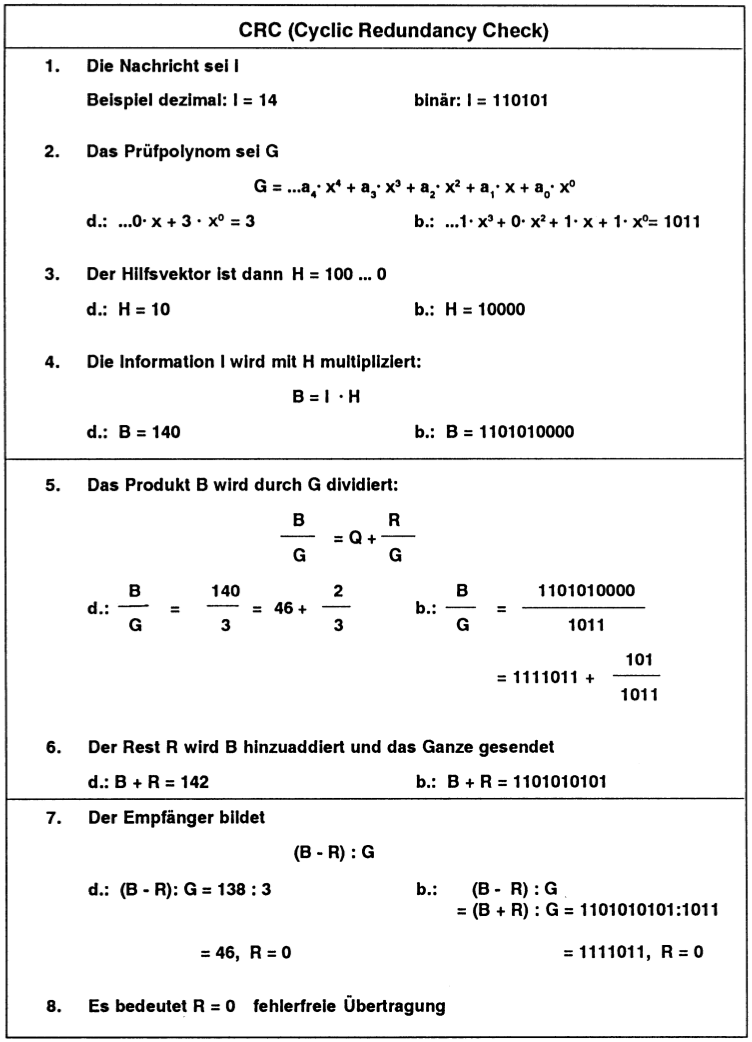
\includegraphics[width=\textwidth]{abbildungen/20160314_crc}
\caption[\textit{Cyclic Redundancy Check}]{\textit{Cyclic Redundancy Check}, entnommen aus \cite[S.~38]{schn06}}
\label{fig:crc}
\end{figure}

Beim sogenannten \acrlong{crc} (\acrshort{crc}) wird ein gesamtes Telegramm als Zahl aufgefasst. Im Sender wird diese Zahl durch ein bestimmtes Generatorpolynom $G$ geteilt. Das Ergebnis wird verworfen, lediglich der Rest bei der Division wird an das Telegramm angehängt. Der Empfänger wiederum dividiert das empfangene Telegramm durch dasselbe Polynom G. Falls sich ein Divisionsrest von 0 ergibt, war die Übertragung fehlerfrei, ansonsten hat sich ein Fehler bei der Übertragung ereignet. Abhängig vom Generatorpolynom G, lassen sich unterschiedliche Güten bei der Fehlererkennung realisieren. In \ref{fig:crc} sind die Vorgänge beim Cyclic Redundancy Check graphisch zusammengefasst.

\subsubsection{Schnittstellen}
\label{sub:schnitt}

Die physikalische Übertragung der Telegramme kann über verschiedenste elektrische oder optische Schnittstellen geschehen und läuft bitweise ab. Je nach Topologie des Bussystems und eingesetztem Übertragungsprotokoll kann die Datenübertragung \textit{seriell} oder \textit{parallel} erfolgen. Bei der parallelen Datenübertragung werden mehrere Bits gleichzeitig übertragen, womit eine hohe Übertragungsgeschwindigkeit erreicht werden kann. Dazu wird eine aufwändige Netzwerktopologie, im Sinne eines vermaschten Netzes, benötigt. Daher erfolgt die Datenübertragung in der Praxis seriell, also einzelne Bits nacheinander über eine gemeinsame Kommunikationsleitung, wie zum Beispiel bei einer Bus-Struktur \cite[S.~13]{sch08}.

\begin{figure}
\centering
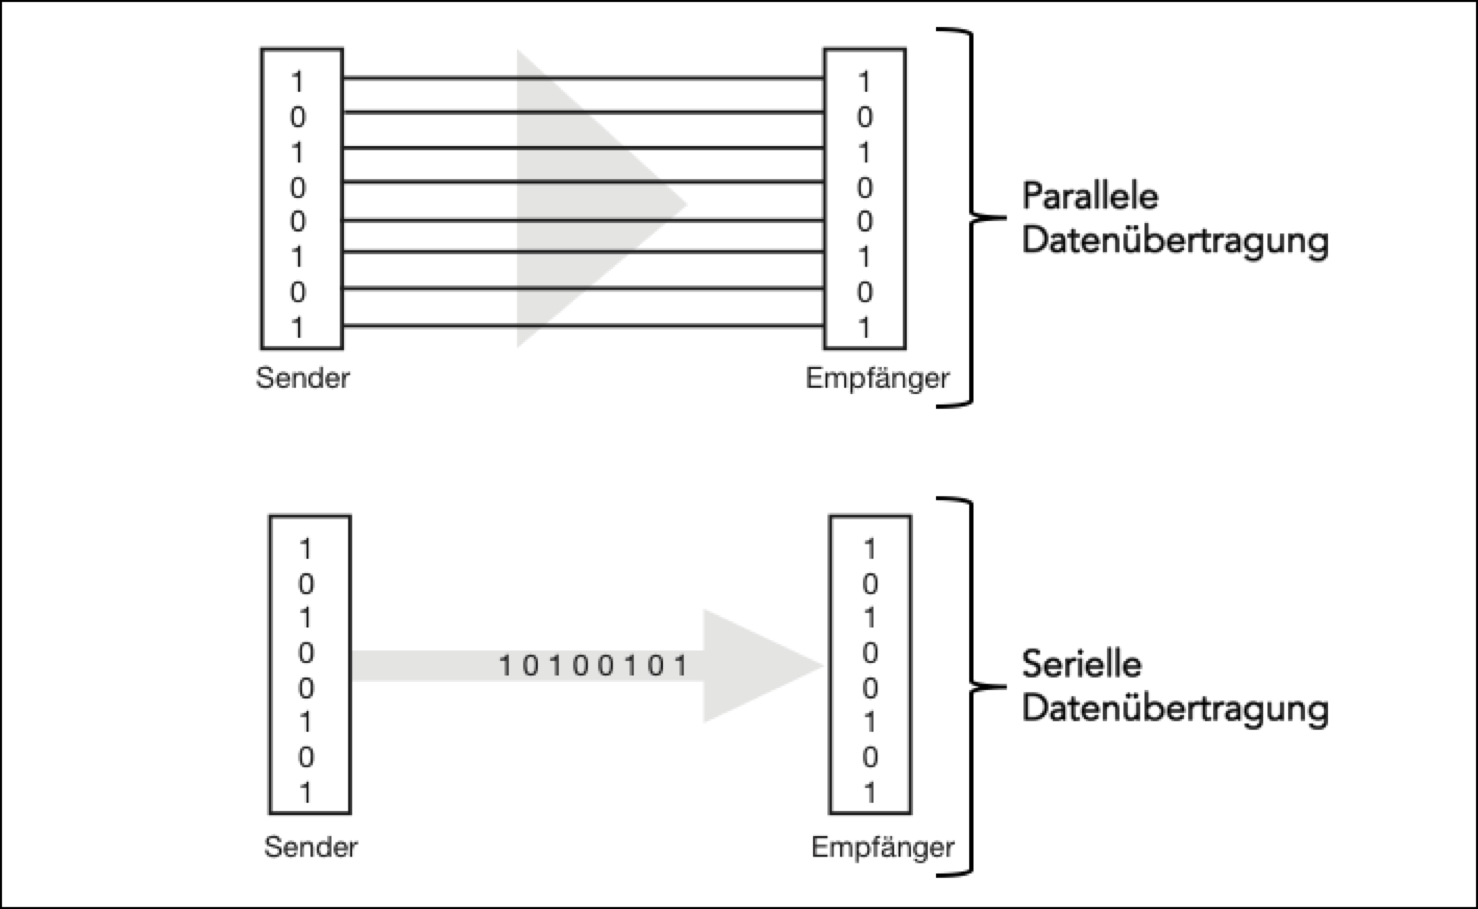
\includegraphics[width=\textwidth]{abbildungen/20160314_seriell}
\caption[Parallele und serielle Datenübertragung]{Parallele und serielle Datenübertragung, entnommen aus \cite[S.~13]{sch08}}
\label{fig:seriell}
\end{figure}


Bei der \textit{binären Datenübertragung} wird lediglich zwischen zwei Zustände unterschieden. Die beiden Zustände werden durch Signalbereiche definiert, welche wiederum durch einen High-Pegel \gls{phigh} und einen Low-Pegel \gls{plow} festgelegt sind. Der Bereich zwischen den beiden Pegeln dient der Hysterese, weshalb der Zustand für Signale in diesem Bereich nicht definiert ist \cite[S.~9]{sch08}.
Die Geschwindigkeit der Datenübertragung wird in übertragenen Bits pro Sekunde $\frac{Bits}{s}$ gemessen und häufig auch als \textit{Baud-Rate} bezeichnet \cite[S.~22]{sch08}.

Die gängigsten Übertragungsverfahren basieren auf elektrischen und optischen Schnittstellen. Die elektrischen Schnittstellen wiederum lassen sich weiter in \textit{Strom-} und \textit{Spannungs-Schnittstellen} untergliedern. Für den weiteren Verlauf der Arbeit sind lediglich die Spannungsschnittstellen \textit{EIA}\footnote{Abkürzung der Normen und Standards die von der Electronic Industries Alliance entwickelt wurden.}\textit{ 232} und \textit{EIA 485} relevant, welche auch als \textit{RS 232} und \textit{RS 485} bezeichnet werden. Nähere Beschreibungen von weiteren wichtigen Schnittstellen sind in \cite[S.~13ff.]{sch08} und \cite[S.~57ff.]{schn06} zu finden.

Die \textit{RS 232 Schnittstelle} ist eine Spannungsschnittstelle, deren definierte Signalpegel in \ref{fig:rs232} zu sehen sind. Die Pegel sind für Spannungen zwischen $3V<p_{high}<15V$ als logische \Gun 1\Gob, der Low-Pegel für Spannungen zwischen $-3V<p_{low}<-15V$ als die logische \Gun 0\Gob definiert. Im Intervall $[-3V,3V]$ ist das Signal nicht definiert, weshalb dieser Bereich möglichst schnell durchlaufen werden sollte. Da der Signalpegel von der Datenleitung hin zur Masse gemessen wird, kann er nicht symmetrisch sein und wird als erdunsymmetrisch bezeichnet. \cite[S.~57f.]{schn06}

\begin{figure}
\centering
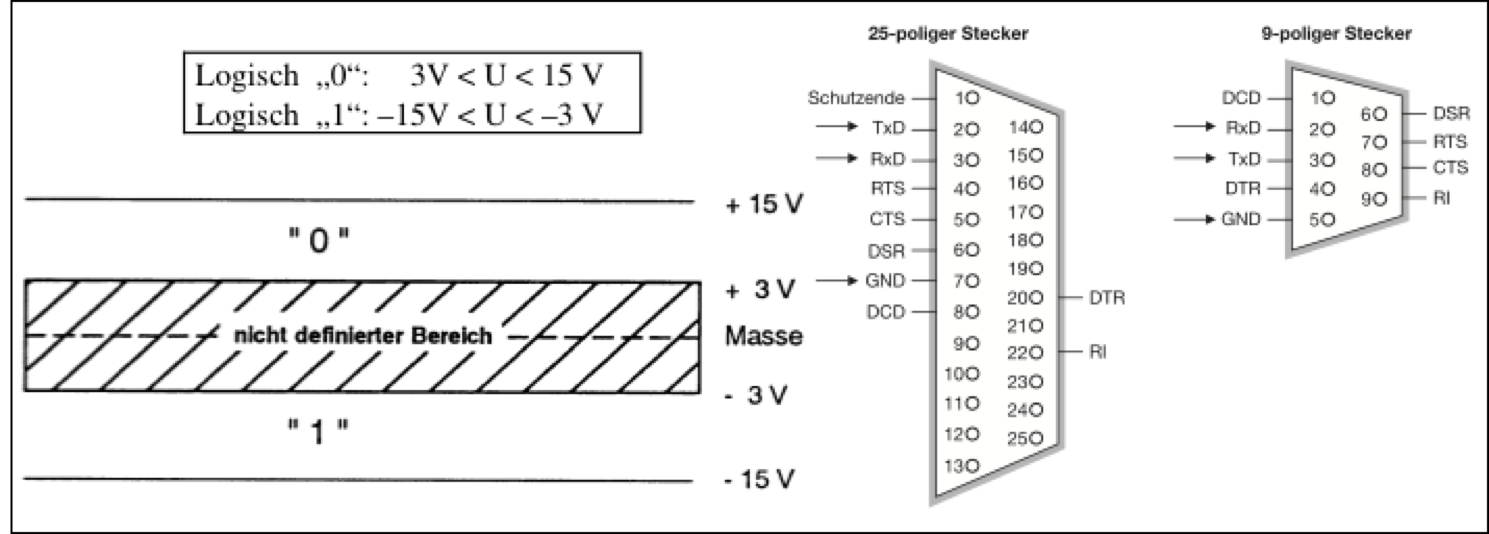
\includegraphics[width=\textwidth]{abbildungen/20160314_rs232}
\caption[Spannungspegel und Stecker der EIA 232-Schnittstelle]{Links: Spannungspegel EIA 232-Schnittstelle, entnommen aus \cite[S.~57]{schn06} \newline Rechts: Stecker EIA 232-Schnittstelle, entnommen aus \cite[S.~14]{sch08}}
\label{fig:rs232}
\end{figure}

Typischerweise steht eine RS 232 Schnittstelle bei handelsüblichen Rechnern als \textit{COM-Port} zur Verfügung. In der Automatisierungstechnik werden zumeist nur die \textit{RxD} (Receive Data), \textit{TxD} (Transmit Data) und \textit{GND}, welche ein gemeinsames Bezugspotenzial definiert, Leitungen verwendet. Wichtig bei der Verkabelung ist, dass die übertragende Leitung TxD mit der empfangenden Leitung RxD verbunden wird \cite[S.~14f.]{sch08}.

Die \textit{RS 485 Schnittstelle} ist ebenfalls eine Spannungsschnittstelle, die in der Norm \textit{ISO 8482} ausführlich beschrieben ist. Die Signalübertragung erfolgt mithilfe von zwei Übertragungsleitungen, die in der Regel als verdrillte und abgeschirmte Zweidrahtleitung ausgeführt sind. Die Signalpegel entsprechen der Differenzialspannung $U_{AB}$ zwischen den beiden Leitungen, die innerhalb des Intervalls von $[-7V,12V]$ liegen muss. Durch das verdrillte Leitungspaar, wirken sich mögliche Störgrößen auf die Spannung beider Leitungen gleichermaßen aus, wodurch die Spannungsdifferenz unverändert bleibt und eine erhöhte Störfestigkeit gegenüber der EIA 232-Schnittstelle erreicht wird.
Bei der Pegelfestlegung werden für Empfänger und Sender verschiedene Vorgaben gemacht, welche in \ref{fig:rs485} graphisch dargestellt sind. So müssen die Sender eine Differenzspannung zwischen $-1,5V<U_{AB}<-5V$ für die logische \Gun 1\Gob und $1,5V<U_{AB}<-5V$ für die logische \Gun 0\Gob leisten können. Empfänger hingegen müssen in der Lage sein, Spannungsdifferenzen von $U_{AB}<-0,3V$ als logische \Gun 1\Gob und $0,3<VU_{AB}$ als logische \Gun 0\Gob zu detektieren \cite[S.~59ff.]{schn06}.

\begin{figure}
\centering
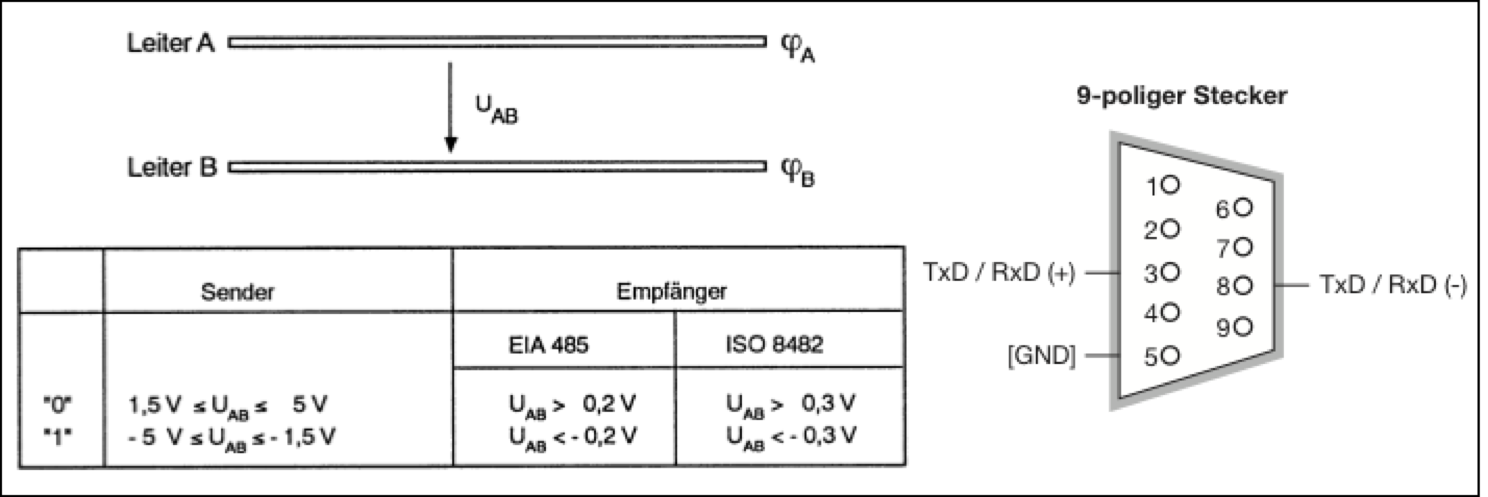
\includegraphics[width=\textwidth]{abbildungen/20160314_rs485}
\caption[Spannungspegel und Stecker der EIA 485-Schnittstelle]{Links: Spannungspegel EIA 485-Schnittstelle, entnommen aus \cite[S.~60]{schn06} \newline Rechts: Stecker EIA 485-Schnittstelle, entnommen aus \cite[S.~19]{sch08}}
\label{fig:rs485}
\end{figure}

Die Datenübertragung erfolgt über die \textit{TxD/RxD+} und \textit{TxD/RxD-} Leitung, ein gemeinsames Bezugspotential über die GND Leitung wird nicht zwingend benötigt. Allerdings wird zusätzlich ein Leitungsabschluss an beiden Enden des Buskabels benötigt.  \cite[S.~19f.]{sch08}.

Um ein Netzwerk zu erweitern, können verschiedene Arten von Bauteile eingesetzt werden. Sogenannte \textit{Repeater} sind aktive Bauteile, die eine kurze Zeitverzögerung verursachen und Netzwerke derselben Schnittstelle miteinander verbinden. Es werden lediglich die einzelnen Leitungen miteinander verbunden und das Datensignal verstärkt, indem die empfangenen Bits blind kopiert und auf das angeschlossene Netzwerksegment übertragen werden. Daher ist er für die Kommunikationsteilnehmer unsichtbar \cite[S.~79f.]{schn06}.

Eine Möglichkeit, um Netzwerke verschiedener Art miteinander zu verbinden, bieten \textit{Bridges} und \textit{Gateways}. Erstere werden auch als \textit{Schnittstellenumsetzer} bezeichnet und kommen zum Einsatz, wenn das gleiche Übertragungsprotokoll bei unterschiedlichen physikalischen Schnittstellen genutzt wird \cite[S.~80f.]{schn06}. Eine Bridge erkennt die Datenflussrichtung automatisch und wandelt die Signale gemäß den Pegeln des jeweils anderen Netzwerks um \cite[S.~21]{sch08}
Die sogenannten Gateways dienen der Kopplung von Netzwerken, die verschiedene Architekturen aufweisen. Sie werden benötigt, falls neben unterschiedlichen physikalischen Schnittstellen auch verschiedene Übertragungsprotokolle verwendet werden. Das Gateway ist demnach umfassender als eine Bridge und erweitert deren Funktionen, um die Übersetzung der Telegramme von einem Übertragungsprotokoll in das jeweils andere \cite[S.~84f.]{schn06}.


\subsection{OSI-Kommunikationsmodell}

Aufgrund der großen Anzahl verschiedener technischer Systeme existieren auch viele verschiedene Arten der Kommunikation untereinander. Bei der genaueren Betrachtung der Kommunikation wird ersichtlich, dass diese oftmals ähnlich abläuft und sich durch ein Meta-Schema beschreiben lässt \cite[S.~8]{schn06}. Um die Kommunikation auch über verschiedenen Systeme hinweg zu ermöglichen und zu formalisieren, wurde von der \acrlong{ios} (\acrshort{ios}) 1984 ein abstraktes Referenz-Modell entwickelt, dass in der \textit{ISO-Norm 7498-1} beschrieben ist. Es dient der Entwicklung und Verbesserung von Standards des Informationsaustausch sowie der Wahrung einer gewissen Konsistenz, als Referenz für bestehende Standards \cite[S.~1]{osi96}. Das Ziel bei dem Entwurf des Modells war es, eine Menge ann Standards zu schaffen, um autonomen Systemen die Kommunikation untereinander zu ermöglichen \cite[S.~4]{osi96}.

Das sogenannte \acrlong{osi} (\acrshort{osi}) wird im Folgenden erläutert, und abschließend im Anwendungskontext der Modbus Kommunikationstechnologie referenziert.

Zunächst wird im Standard definiert, womit sich das Modell beschäftigt und abgegrenzt, welche Aspekte im Modell keine Berücksichtigung finden \cite[S.~3]{osi96}:
\begin{quote}
\textit{\Gun OSI is concerned with the exchange of information between open systems (and not the internal functioning of each individual real open system).\Gob}
\end{quote}

Das \acrshort{osi} beschäftigt sich also zentral mit dem Austausch von Informationen zwischen verschiedenen offenen Systemen und allen dabei anfallenden Aktivitäten. Diese sind sehr umfangreich und lassen sich in folgenden vier Bereiche gliedern \cite[S.~3f.]{osi96}:
\begin{itemize}
	\item Der Austausch von Informationen zwischen offenen Systemen,
	\item die physischen Medien zur Verbindung von offenen Systemen und deren Gegebenheiten zum Transport von Informationen,
	\item die Vernetzung von offenen Systemen
	\item sowie die Interaktion zwischen offenen Systemen und deren Fähigkeit zur Kooperation bei der Datenübertragung.
\end{itemize}
Bezogen auf den Austausch von Informationen, überschneidet sich die physische Verbindung und die Vernetzung zur Infrastruktur und Architektur. Diese steht dann für die Übertragung zur Verfügung steht. Die Interaktion umfasst weitaus mehr Aufgaben: Neben der Synchronisation der Prozesse, welche Daten austauschen wollen, muss auch die Darstellung der Daten und eventuell notwendige Transformationen beachtet werden, um eine Kompatibilität unterschiedlicher Systeme zu erreichen. Weitere wichtige Aufgaben sind die Datenspeicherung und i-ntegrität sowie die Sicherheit beim Austausch hinsichtlich Fehlern und Datenschutz \cite[S.~4]{osi96}.
Es ist leicht zu erkennen, dass die technische Kommunikation einen sehr umfangreichen und komplizierten Prozess darstellt. Daher wird der Kommunikationsprozess im \acrshort{osi} stark abstrahiert und in sieben gedankliche Ebenen gegliedert. Die einzelnen abstrakten Ebenen sind in \ref{fig:osi} dargestellt und fassen verschiedene Aufgaben des Kommunikationsprozesses in Teilaufgaben zusammen.

\begin{figure}
\centering
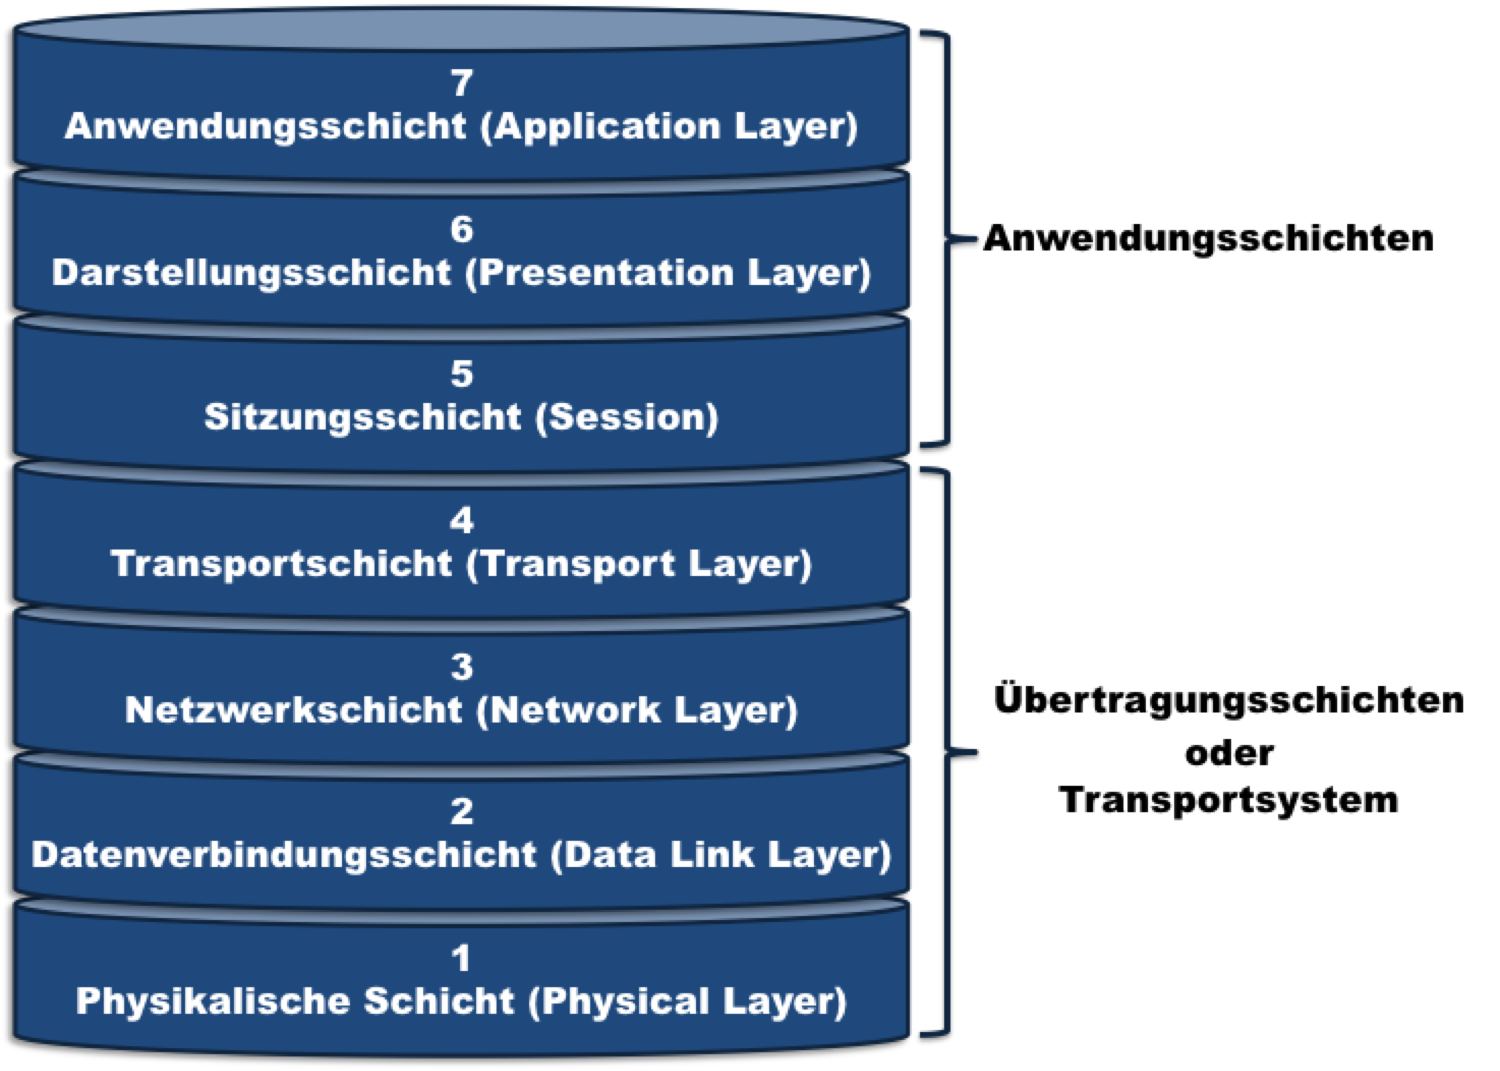
\includegraphics[width=\textwidth]{abbildungen/20160112_osi}
\caption[Die sieben Schichten des Open System Interconnection Modells]{Die sieben Schichten des \textit{Open System Interconnection} Modells, verändert nach \cite[S.~10]{schn06} und \cite[S.~28]{osi96}}
\label{fig:osi}
\end{figure}


Die Ebenen werden als Schichten bezeichnet und haben klar definierte Aufgaben und Schnittstellen zu ihren Nachbarschichten. An diesen Schnittstellen werden Dienste bereitgestellt, die von den anderen Ebenen genutzt werden können. Durch diesen Aufbau können einzelne Schichten einfach bearbeitet oder ausgetauscht werden, ohne die Gesamtfunktionalität zu gefährden. Außerdem kann ein System auch aus Komponenten verschiedener Hersteller zusammengesetzt werden, wodurch diese Architektur sehr gut als Basis für offene Systeme dient. In \ref{fig:osi} ist ebenfalls dargestellt, dass die Schichten eins bis vier gemeinsam auch als Übertragungsschichten beziehungsweise Transportsystem zusammengefasst werden, weil sie die Aufgabe der Datenübertragung zwischen Systemen übernehmen. Die Schichten fünf bis sieben werden als Anwendungsschichten bezeichnet, weil sie bei der Datenübertragung die Zusammenarbeit zwischen der Anwendersoftware und dem Betriebssystem sicherstellen \cite[S.~8f.]{schn06}.

Die Schnittstellen zwischen den Schichten werden als\textit{ Service Access Points} (SAP) bezeichnet und besitzen jeweils eine eindeutige Adresse. Die obere Schicht ist der \textit{Service User}, der den Dienst der darunter liegenden Schicht nutzt, dem \textit{Service Provider}. Für den Datenaustausch stehen Dienste zur Verfügung, welche in verbindungsorientierte und verbindungslose unterschieden werden. Verbindungslose Dienste benötigen keine Verbindung zwischen den Kommunikationspartnern zur Datenübertragung. Verbindungsorientierte Dienste benötigen für den Datenaustausch zunächst einen virtuellen Kanal zwischen Kommunikationspartnern. Typische Dienste sind beispielsweise das Aufbauen und Abbauen von Verbindungen sowie der eigentliche Datenaustausch \cite[S.~11f.]{schn06}.

Bei der Abhandlung der Dienstaufgaben anhand der Client/Server-Architektur, stehen vier grundlegende Dienstvorgänge zur Verfügung, die zusammengefasst in \ref{fig:vorgang} abgebildet sind \cite[S.~2f.]{mod06tcp}:

\begin{itemize}
	\item Das Stellen einer Anforderung, ein Request,
	\item das Senden einer Meldung, eine Indication,
	\item das Senden eine Antwort, eine Response,
	\item und das Senden einer Bestätigung, eine Confirmation.
\end{itemize}

\begin{figure}
\centering
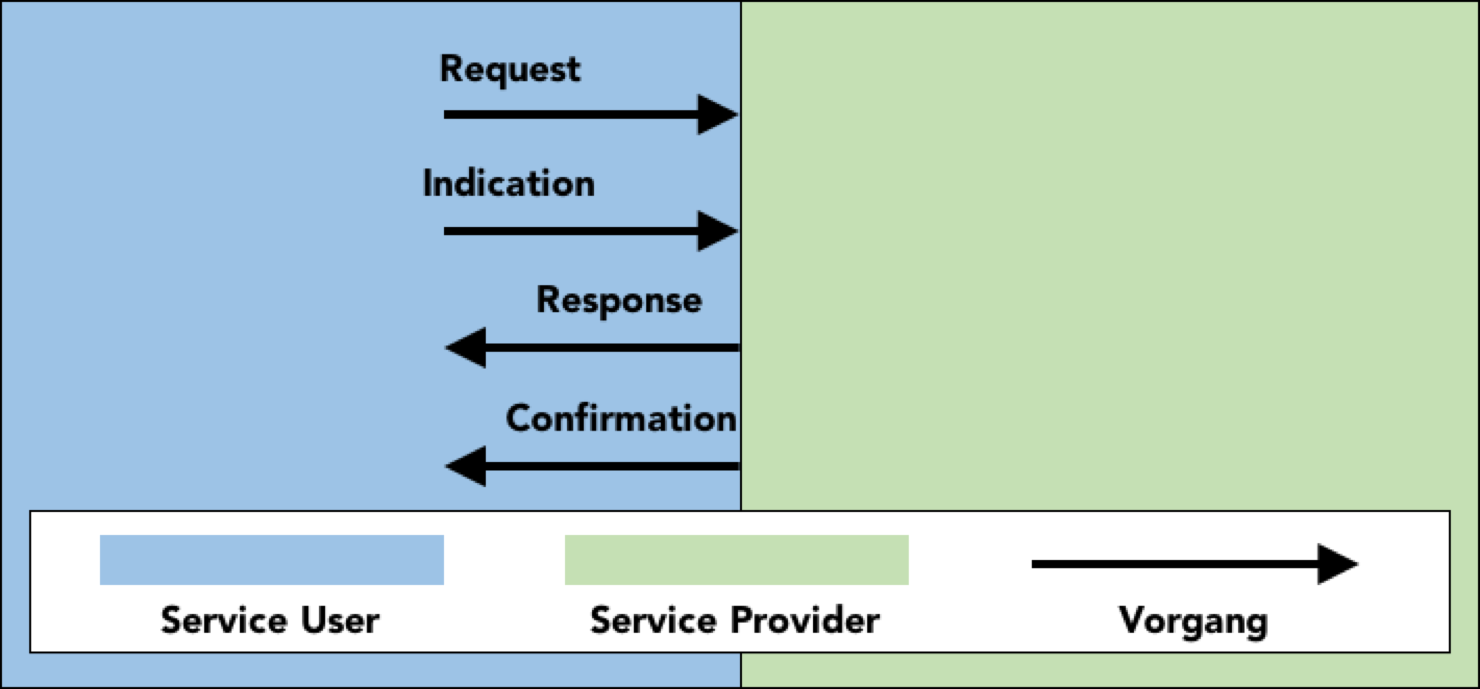
\includegraphics[width=\textwidth]{abbildungen/20160310_vorgang}
\caption{Die vier Dienstvorgänge}
\label{fig:vorgang}
\end{figure}

Die unterste physikalische Schicht definiert die mechanischen und elektrischen Schnittstellen zur physischen Verbindung von Systemen und zur Übertragung der einzelnen Bits \cite[S.~49f.]{osi96}. Sie legt also die mechanischen und elektrischen Eigenschaften der Übertragung fest, also die Endsystemkopplung durch Stecker, die Kabelspezifikationen und die Zuordnung der Anschlüsse. Außerdem wird die Art der Codierung und die Spannungspegel der Übertragung spezifiziert. In der Regel werden dazu bestehende Normen genutzt, wie zum Beispiel die zuvor beschriebene elektrische Übertragungsstrecke nach EIA 485-Norm \cite[S.~14f.]{schn06}.
Ein wichtiger der Ebene ist es, dass die Spezifikation der Schnittstelle und nicht das physikalisches Medium selbst Teil der Schicht eins ist, da die Kommunikation unabhängig von der konkreten Ausprägung abläuft \cite[S.~9]{schn06}.

Die zweite Schicht widmet sich der Kommunikation zwischen zwei Systemen. Deshalb stellt die Datenverbindungsschicht funktionale und prozedurale Hilfsmittel für den Aufbau und die Trennung einer Verbindung sowie den Transfer von Dateneinheiten zur Verfügung. Außerdem  wird der darüber liegenden Netzwerkschicht eine Kontrolle über die Verbindung von physikalischen Netzwerken ermöglicht \cite[S.~46f.]{osi96}.
Eine weitere umfangreiche Aufgabe ist die Sicherung der Daten. Durch die Einteilung der Daten in Rahmen und und die Nutzung von Strategien zur Fehlererkennung und -vermeidung, soll die Sicherheit gewährleistet werden. Dies kann durch die zuvor beschriebenen Methodiken, wie beispielsweise dem CRC geschehen. Wichtig hierbei ist, dass die Schicht keinerlei Kenntnis über Inhalte der Daten hat \cite[S.~9ff.]{schn06}

Die dritte Schicht beschäftigt sich mit dem Netzwerk als Ganzes. Die Aufgaben der Netzwerkschicht hängen davon ab, ob der Datenaustausch  verbindungsorientiert oder verbindungslos stattfindet. Daher steuert sie den Aufbau, die Erhaltung und das Trennen von Verbindungen  sowie den eigentlichen Datenaustausch \cite[S.~41f.]{osi96}. Weiterhin ist sie für den Transport der Daten innerhalb des Netzwerks zuständig. Sie kontrolliert den Datenverkehr im Netzwerk und legt eventuell Routen für die einzelnen Kommunikationsvorgänge fest \cite[S.~11f.]{schn06}.

Die vierte Schicht ist die Transportschicht und ist zuständig für eine transparente Übertragung der Daten. Sie beschäftigt sich nicht mit Transportrouten oder der Verlässlichkeit der Datenübertragung, sondern hat das Ziel einer optimalen Nutzung der Services der darunter liegenden Netzwerkschicht \cite[S.~37f.]{osi96}.
Typische Aufgaben sind die Adressierung der Teilnehmer, der Auf- und Abbau von Transportverbindungen sowie die Synchronisierung der datenaustauschenden Systeme. Außerdem werden die Daten aus der Sitzungsschicht in transportierbare Einheiten zerlegt \cite[S.~12f.]{schn06}.

Die fünfte Schicht -- die Sitzungsschicht -- startet eine Sitzungsverbindung mit eindeutiger Adresse, wenn diese von einer höheren Schicht angefordert wird. Diese Verbindung dient dazu, den Datenaustausch auf höherer Ebene zu organisieren, indem Sitzungsadressen mit den Transportadressen verknüpft werden \cite[S.~35]{osi96}. Sie verbindet demnach die Anwendungsschichten mit dem Transportsystem über eine Schnittstelle \cite[S.~13]{schn06}.

Die sechste Schicht ist nach \cite[S.~33f.]{osi96} mit der Darstellung der Daten betraut, die von beiden Kommunikationsanwendungen entweder verstanden oder referenziert werden. Dadurch wird eine gemeinsame Repräsentation der zu übertragenen Daten geschaffen. \cite[S.~13f.]{schn06} stellt fest, dass diese Dienste eine Syntaxfreiheit der Daten beim Nachrichtenaustausch schaffen und durch eine Kompression der Daten Zeit- und Kostenvorteile der Übertragung generiert werden.

Die siebte und letzte Schicht stellt einem Benutzer lediglich eine Zugriffsmöglichkeit auf das OSI Kommunikationssystem zur Verfügung \cite[S.~32]{osi96}. Benutzer sind in der Regel Softwareanwendungen kein Mensch ist. \cite[S.~14]{schn06}

Im nachfolgenden Abschnitt werden die später angewandten Modbus Protokolle und deren Spezifikation beschrieben und in Bezug zum \acrshort{osi} gebracht, um den praktischen Nutzen davon zu verdeutlichen.


\subsection{Modbus Kommunikationstechnologie}
\label{sub:modbus}

Zunächst wird die Modbus Technologie in das \acrlong{osi} eingeordnet, bevor eine Beschreibung der genauen Spezifikationen und Protokolle anhand der zuvor dargelegten Merkmalen erfolgt.

Das Modbus Protokoll teilt sich in verschiedene Protokolle auf, zum einen auf das \textit{Application Layer Messaging Protocol} auf oberster Ebene, welches auf das \textit{Modbus Over Serial Line Protocol} sowie das \textit{Ethernet} und \textit{TCP/IP Protokoll} aufbauen kann.
Das Application Layer Messaging Protocol lässt sich im OSI Referenzmodell in die siebte und oberste Schicht(Anwendungsschicht) einordnen wie in \ref{fig:modbusosi} dargestellt. Bei der gemeinsamen Nutzung mit dem Modbus Over Serial Line Protocol, wird letzteres in die zweite Schicht eingeordnet und die Ebenen drei bis sechs sind leer implementiert. Als physikalische Schicht werden die Übertragungsstandards nach EIA 485 oder nach EIA 232 genutzt \cite[S.~2]{mod06ser}.

Anstatt des seriellen Modbus Protkolls kann auch das \textit{Modbus Messaging On TCP/IP Protocol} verwendet werden, dass dabei zusammen mit den dem TCP/IP Protokoll zusammen die Netzwerkschicht im OSI-Referenzmodell implementiert. Die Ethernet Technologie implementiert dann die Datensicherungsschicht und definiert die Spezifikationen der untersten physikalischen Schicht und deren Schnittstellen. Die Ebenen vier bis sechs sind auch bei Nutzung dieser Kommunikationsweise leer implementiert \cite[S.~2f.]{mod12}. Eine allgemeine Einführung zur Ethernet Technologie und zum TCP/IP Standard findet sich in \cite{schn06}. Für eine ausführliche Darstellung wird jedoch auf \cite{fu03} verwiesen.

Die Funktionen der einzelnen Ebenen werden im folgenden ausführlich dargestellt. Zunächst wird das Modbus Application Layer Messaging Protocol erläutert, dass von beiden unteren Modbus Protokollen genutzt wird. Anschließend werden letztere bis hin zu den physikalischen Schnittstellen erläutert.

\begin{figure}
\centering
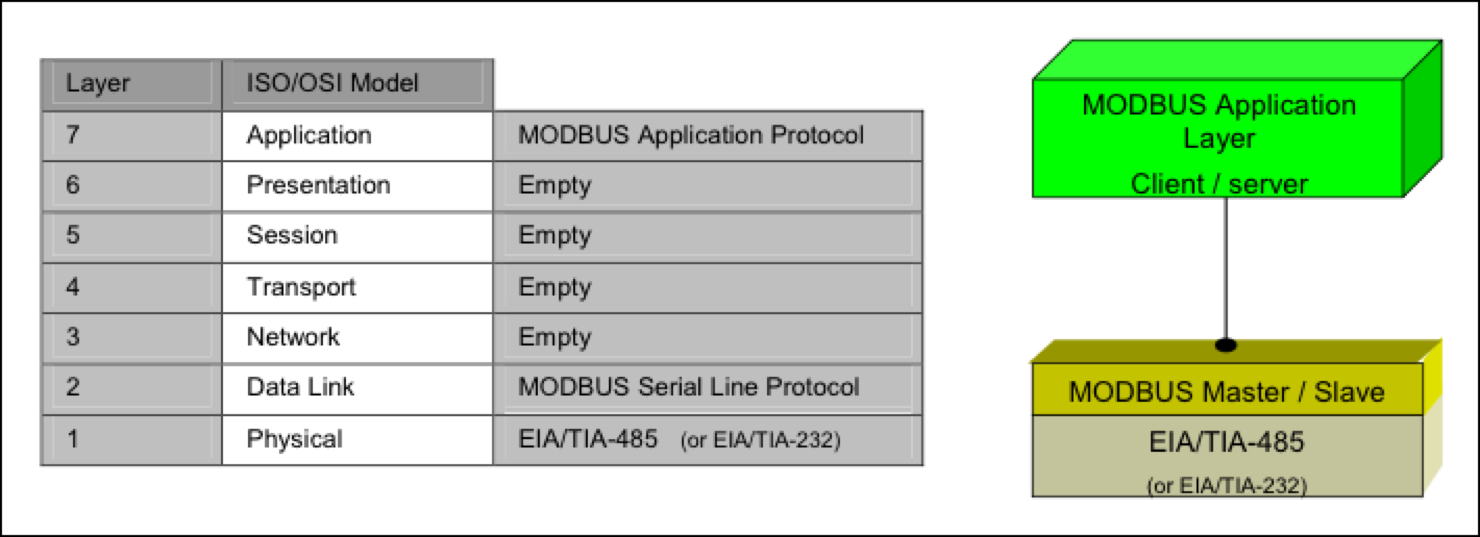
\includegraphics[width=\textwidth]{abbildungen/20160319_modbusosi}
\caption[Die Modbus Kommunikation im OSI-Referenzmodell]{Die Modbus Kommunikation im OSI-Referenzmodell, entnommen aus \cite[S.~5]{mod06ser}}
\label{fig:modbusosi}
\end{figure}

Das Modbus Application Layer Messaging Protocol kann von verschiedenen Netzwerken und Bussystemen zur Master/Slave Kommunikationen genutzt werden \cite[S.~2f.]{mod12}.
Das Protokoll definiert eine gemeinsame Telegrammstruktur, bezogen auf die Inhalte und den Rahmen des Telegramms. Diese Definition ermöglicht die Kommunikation zwischen verschiedenen Geräten innerhalb eines Netzwerks, unabhängig von Art und Typ des darunter liegenden Netzwerks. Es beschreibt außerdem wie die Kommunikation abläuft. Zum einen, wie der Master beziehungsweise Client eine Anfrage an einen Server beziehungsweise Slave stellt, zum anderen deren Reaktionen und Antworten auf Anfragen. Außerdem beschreibt es die Überwachung auf Übertragungsfehler \cite[S.~2f.]{mod96}.
Die Kommunikation kann über eine serielle Leitung nach EIA 485 beziehungsweise EIA 232 sowie über ein lokales Ethernet-Netzwerk erfolgen. Über Gateways, wie in Abschnitt \ref{sec:grundlagenbus} erläutert, kann die Kommunikation auch über verschiedene Typen von Bussystemen oder Netzwerken geschehen \cite[S.~3f.]{mod12}.

Das allgemeine Gerüst für Modbus Telegramme ist in \ref{fig:modbusframe} dargestellt. Die Protocol Data Unit (PDU) enthält die auszutauschenden Informationen und ist unabhängig vom Netzwerk oder dem Bussystem. Zu den Informationen zählen die eigentlichen Daten, welche auch leer sein können, sowie ein Funktionscode, der beschreibt welche Art der Reaktion gefordert wird. Die sogenannte Application Data Unit (ADU) enthält neben der PDU weitere Informationen zur Adressierung im Netzwerk und zur Fehlererkennung und ist daher abhängig von der zugrundeliegenden Netzwerkstruktur.

\begin{figure}
\centering
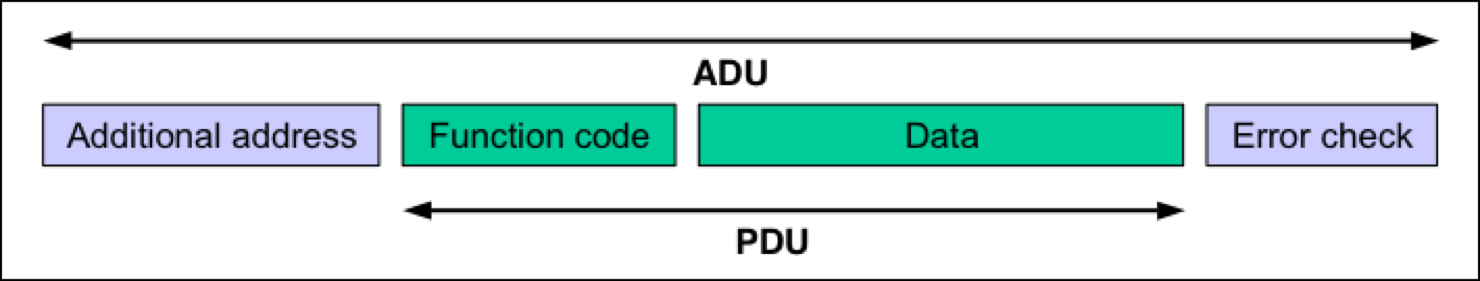
\includegraphics[width=\textwidth]{abbildungen/20160319_Modbusframe}
\caption[Allgemeiner Rahmen für Telegramme nach dem Modbus Anwendungsprotokoll]{Allgemeiner Rahmen für Telegramme nach dem Modbus Anwendungsprotokoll, entnommen aus \cite[S.~3]{mod12}}
\label{fig:modbusframe}
\end{figure}

Die Kommunikation erfolgt anhand einer \textit{Server/Client Architektur}, bei der der \textit{Client} die Rolle des Masters und die \textit{Server} die Rolles der Slaves übernehmen. Sie wird innerhalb des Clients durch eine ADU initialisiert. Das genaue Format der ADU wird durch die Wahl des Modbus RTU oder TCP Protokolls festgelegt. Das Schema einer Transaktion läuft jedoch bei beiden nach demselben Prinzip ab, welches in \ref{fig:modbustransaktion} graphisch dargestellt ist.
Wenn eine ADU fehlerfrei empfangen wurde nutzt der Server den Funktion Code, um anzuzeigen ob ein Fehler aufgetreten ist. Ist die der Fall, wird dies durch einen Exception Function Code angezeigt. Ansonsten sendet der Server eine normale Antwort, zusammen mit einem einfachen Echo des empfangenen Funktionscodes.
Die Größe der PDU ist aufgrund der seriellen Kommunikation begrenzt auf 256 Bytes. Da zwei Bytes für einen Cyclic Redundancy Check und ein Byte für die Server Adresse reserviert sind, ist die PDU auf eine Länge von 253 Bytes begrenzt.

Ein weiterer, wichtiger Aspekt ist, dass das Modbus Anwendungsprotokoll die \Gun big-Endian\Gob Codierung für Daten verwendet verwendet, deren numerischer Wert größer als ein einzelnes Byte ist \cite[S.~3ff.]{mod12}. 
Anhand des Beispiels einer Uhrzeit, kann die Bedeutung der Big-Endian Repräsentation einfach erläutert werden: Die Daten werden zum Transport so aufgeteilt, dass zunächst die Daten mit der höchsten Wertigkeit, also den Stunden zuerst gesendet werden. Anschließend folgen die Minuten und zum Schluss die Sekunden, unabhängig von deren numerischem Wert. Werden nun nacheinander die Telegramme $03$, $50$, $12$ empfangen, werden diese als 03:50:12h interpretiert. Der interessierte Leser wird für nähere Ausführungen, auch zu little-Endian Codierung, an \cite{endian05} verwiesen.

\begin{figure}
\centering
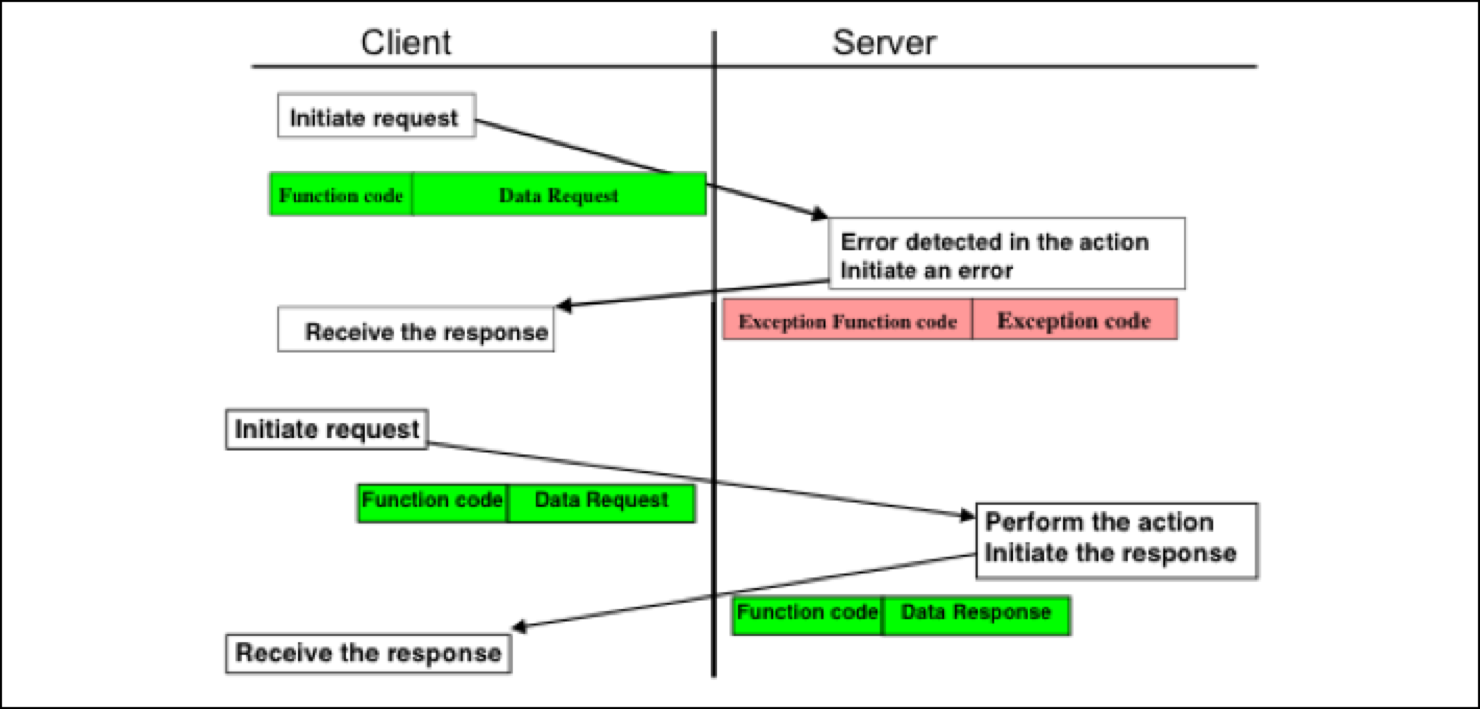
\includegraphics[width=\textwidth]{abbildungen/20160319_modbusclientserver}
\caption[Transaktion mit dem Modbus Protokoll]{Transaktion mit dem Modbus Protokoll, nach \cite[S.~4]{mod12}}
\label{fig:modbustransaktion}
\end{figure}

Die Funktionscodes umfassen ein Byte und sind wie bereits angesprochen in der PDU enthalten. Es existieren 255 verschiedene Codes die von 1 aufwärts gezählt werden. Sie definieren welche Aktion ein Server ausführen soll. In erster Linie dienen sie dem Datenzugriff in verschiedenen Tabellen, können aber auch für Diagnosen oder nutzerdefinierte Aktionen benutzt werden. Weiterhin lassen sie sich in drei große Gruppen untergliedern, die öffentlichen, nutzerdefinierbaren und die reservierten Funktionscodes. Die öffentlichen Codes sind wohldefiniert und dokumentiert sowie auf Konformität getestet und sind daher einfach, schnell und sicher nutzbar. Die vom nutzerdefinierbaren Funktionscodes können genutzt werden um die öffentlichen Codes durch eigene Funktioniltäten zu ergänzen. Die reservierten Codes sind für Altprodukten einiger Unternehmen reserviert, welche an der Entwicklung des Modbus Protokolls beteiligt waren \cite[S.~10ff.]{mod12}.

Das Modbus Datenmodell basiert darauf, dass durch den Funktionscode und auf die Daten in vier verschiedenen Tabellen für unterschiedliche Funktionen und Datenobjekte zugegriffen werden kann:
\begin{itemize}
	\item In die \textit{Discretes Input} Tabelle, welche Single Bit Objekte enthält und lediglich gelesen werden kann,
	\item die \textit{Coils} Tabelle, welche ebenfalls Single Bit Objekte enthält jedoch gelesen und beschrieben werden darf,
	\item die \textit{Input Registers} Tabelle, die Datenobjekte als 16-Bit Wort enthält und wiederum nur gelesen werden kann
	\item und die \textit{Holding Registers} Tabelle, dessen 16-Bit Wort Objekte wiederum gelesen und beschrieben werden dürfen.
\end{itemize}

Ein 16-Bit Wort entspricht einer Folge von 16 binären Symbolen. Nach der \textit{IEC 61131-3 Norm} entspricht es im Rechner einem Integer Wert und es lassen sich damit ganze Zahlen zwischen 0 und 65.536 beziehungsweise -32.768 und 32.767 darstellen.
Die Daten selbst können auch innerhalb einer einzigen Tabelle abgelegt sein, es muss lediglich Interface für den Zugriff auf die vier verschiedenen Tabellen möglich sein. Jede Tabelle ist begrenzt auf maximal 65536 Einträge, deren Adressierung bei beginnt 0 und bei 65535 endet \cite[S.~6ff.]{mod12}. An welcher Stelle welche Daten zu finden wird vom Hersteller eines modbusfähigen Geräts definiert und üblicherweise durch ein Modbusadressmapping beschrieben. Ein Beispiel dazu findet sich in den Datenblätter zu den Komponenten der Anlage in Anhang \ref{att:modbusmap}.
Um also auf die Daten einer modbusfähigen Komponente zugreifen zu können, muss durch den Funktionscode die richtige Tabelle und durch die Adresse wiederum die richtige Stelle in der Tabelle referenziert werden.

\begin{figure}
\centering
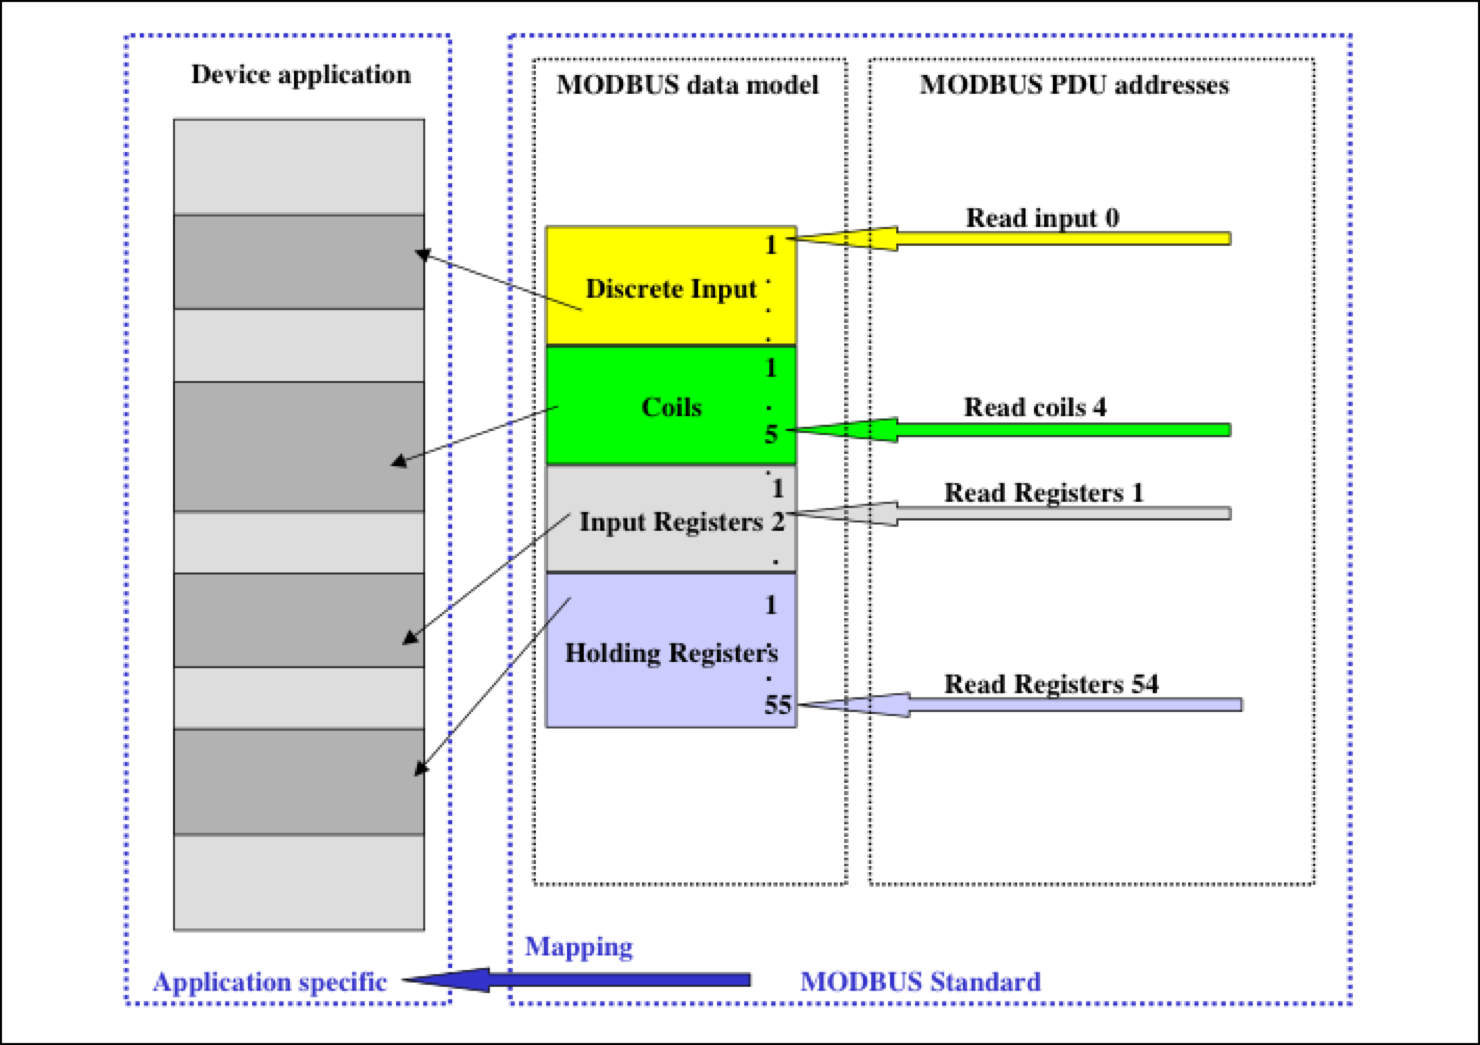
\includegraphics[width=\textwidth]{abbildungen/20160319_modbusadresse}
\caption[Datenmodell und Adressierung nach dem Modbus Protokoll]{Datenmodell und Adressierung nach dem Modbus Protokoll, entnommen aus \cite[S.~8]{mod12}}
\label{fig:modbusadresse}
\end{figure}

Beim \textit{Modbus Over Serial Line Protocol} können die Daten über zwei unterschiedliche Modi übertragen werden, dem \textit{RTU} und \textit{ASCII Modus}. Der ASCII Modus stellt eine exotische Anwendung dar und wird in \cite{mod06ser} detailliert beschrieben.
Der RTU Modus findet bei der Kommunikation der Anlage in Kapitel \ref{chap:anlagendesign} Anwendung und wird von allen seriellen modbusfähigen Komponenten unterstützt.
Das Protokoll spezifiziert das folgende Format zur Übertragung der einzelnen Bytes: Jede Byteübertragung beginnt mit einem \textit{Startbit}, auf dass dass zu übertragende Byte, bestehend aus acht einzelnen Bits, folgt. Abgeschlossen wird die Übertragung optional von einem \textit{Paritätsbit} und einem \textit{Stoppbit} beziehungsweise lediglich von zwei StoppBits. Dabei wird jedes zu übertragende Byte als zwei 4-bit hexadezimales Zeichen übertragen \cite[S.~12f.]{mod06ser}. Die Paritätsprüfung ist optional und dient der Fehlerüberprüfung bei der Byteübertragung, wie bereits zuvor in Abschnitt \ref{sec:grundlagenbus} erläutert. Eine graphische Darstellung dieses Vorgangs findet sich in \ref{fig:modbusrtu}.
Der \textit{Rahmen} eines Modbus RTU Telegramms besteht aus der \textit{Slave Adresse}, die für jeden Slave innerhalb eines Netzwerks eindeutig ist und einen numerischen Wert zwischen 1 und 247 besitzt. Anschließend folgt der \textit{Function Code}, der den Tabellenzugriff definiert. Darauf folgen die eigentlichen Informationen für die 0 bis maximal 252 Bytes vorgesehen sind. Abgeschlossen wird der Rahmen durch ein \textit{CRC Feld} zur Fehlerüberprüfung. Der Ablauf und die Vorgänge des CRC Checks beim RTU Protokoll sind detailliert in \cite{mod06ser} beschrieben. Die Übertragung eines Telegramms erfolgt byteweise, wie zuvor beschrieben. Die Datensicherung findet also durch eine Paritätsprüfung und einen CRC auf verschiedenen Ebenen statt.
Die \textit{Übertragungszeit} eines Bytes und eines Telegramms hängt wiederum von der \textit{Baudrate} ab. Um den Beginn und den Abschluss eines RTU Rahmens eindeutig zu definieren, geschieht dies in Abhängigkeit von der Baudrate. Zwischen einzelnen Bytes folgt ein stilles Intervall, dass je nach Länge angibt, ob das Telegramm beendet ist oder fortgesetzt wird. Auf ein stilles Intervall das kleiner oder gleich der anderthalbfachen Übertragungszeit eines Bytes ist, folgt eine weiteres Byte. Ist das stille Intervall länger als die dreieinhalbfache Byteübertragungszeit markiert dies das Ende eines Telegramms und den Beginn des nächsten Telegramms \cite[S.~13]{mod06ser}. Diese Zusammenhänge sind zur Veranschaulichung in \ref{fig:modbusrtu} zusammengefasst.

\begin{figure}
\centering
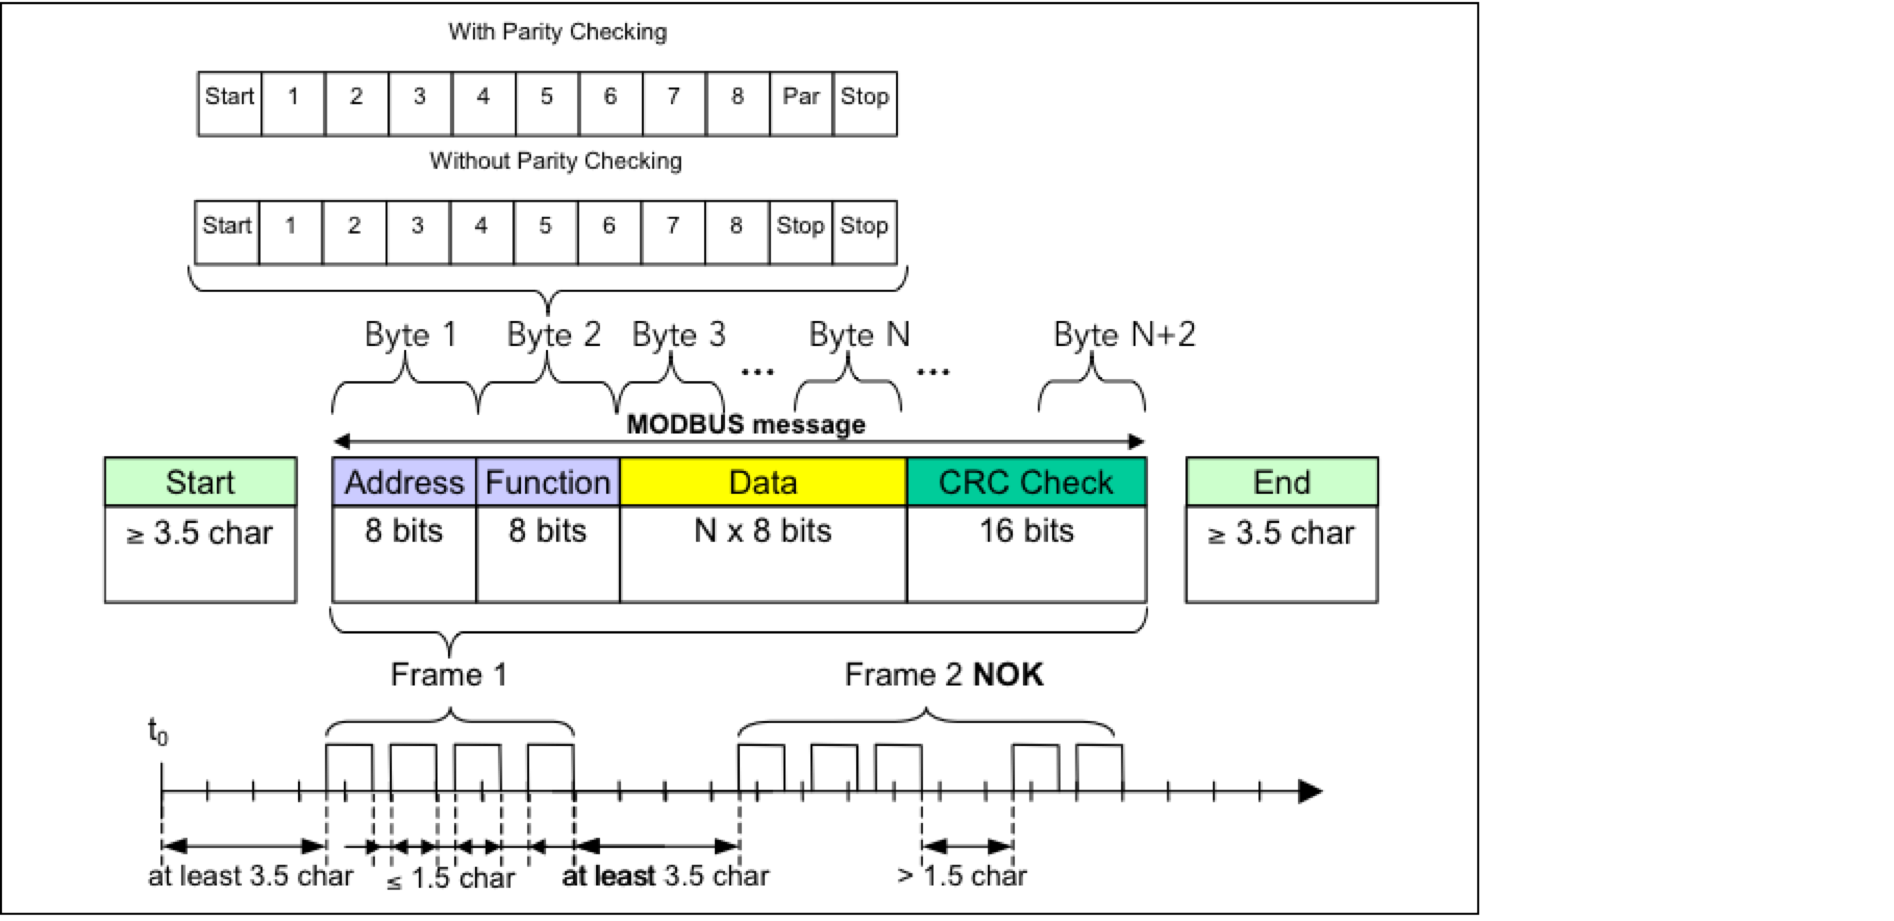
\includegraphics[width=\textwidth]{abbildungen/20160321_rtu}
\caption[Serielle Kommunikation über Modbus RTU]{Serielle Kommunikation über Modbus RTU, nach \cite[S.~12f.]{mod06ser}}
\label{fig:modbusrtu}
\end{figure}

Der Implementierungsleitfaden innerhalb des Protokolls legt auch die Spezifikationen der physikalischen Schicht fest, die im Folgenden beschrieben werden.
Er wird eine EIA~483 Schnittstelle als elektrisches Interface vorgeschlagen, erlaubt aber weiterhin die Nutzung einer EIA~232 Schnittstelle zur Datenübertragung. Bei beiden erfolgt die Datenübertragung über ein verdrilltes Leiterpaar. Weiterhin wird eine Baudrate von 9.600 und 192.000 bei einer Even Parität als \textit{Standardkonfiguration} des seriellen Netzwerks festgelegt. Die Verkabelung der Komponenten erfolgt bei beiden elektrischen Standards standmäßig durch ein verdrilltes Leiterpaar und einer gemeinsamen Verbindungsleitung. Die beiden Leitungen des verdrillten Paares werden mit \textit{D1}, welche auch \textit{D+} oder \textit{Modbus A} Leitung genannt wird, und \textit{D0}, welche auch \textit{D-} oder \textit{Modbus B} Leitung genannt wird, bezeichnet. Ein Standard-Netzwerk besteht aus maximal 32 Teilnehmern, dass durch den Einsatz von Repeatern vergrößert werden kann. Das Netzwerk wird durch eine Bus-Struktur ausgeführt, nach der die einzelnen Komponenten im Netzwerk angeordnet werden. Die beiden Enden der Busleitung werden durch einen Widerstand von $150 Ohm$ zwischen der D0 und D1 Leitung abgeschlossen \cite[S.~20ff.]{mod06ser}.
Die Verbindung der Kabel kann im einfachsten Fall durch einfache Schraubklemmen erfolgen, jedoch können auch genormte mechanische Interfaces genutzt werden, deren Ausführung und Verkabelung in \cite[S.~29ff.]{mod06ser} detailliert beschrieben sind.

Das \textit{Modbus Messaging on TCP/IP Protocol} ermöglicht die Kommunikation von Geräten, die über ein Ethernet miteinander verbunden sind. Des Weiteren ermöglicht dieses Protokoll explizit Netzwerksegmente über Bridges, Gateways oder Router Netzwerke miteinander zu verbinden. Das Protokoll erlaubt das Einbinden serieller Netzwerksegmente und eine übergreifende Kommunikation \cite[S.~2f.]{mod06tcp}. Eine beispielhafte Kommunikationsarchitektur ist in \ref{fig:tcparchiktektur} dargestellt. 

\begin{figure}
\centering
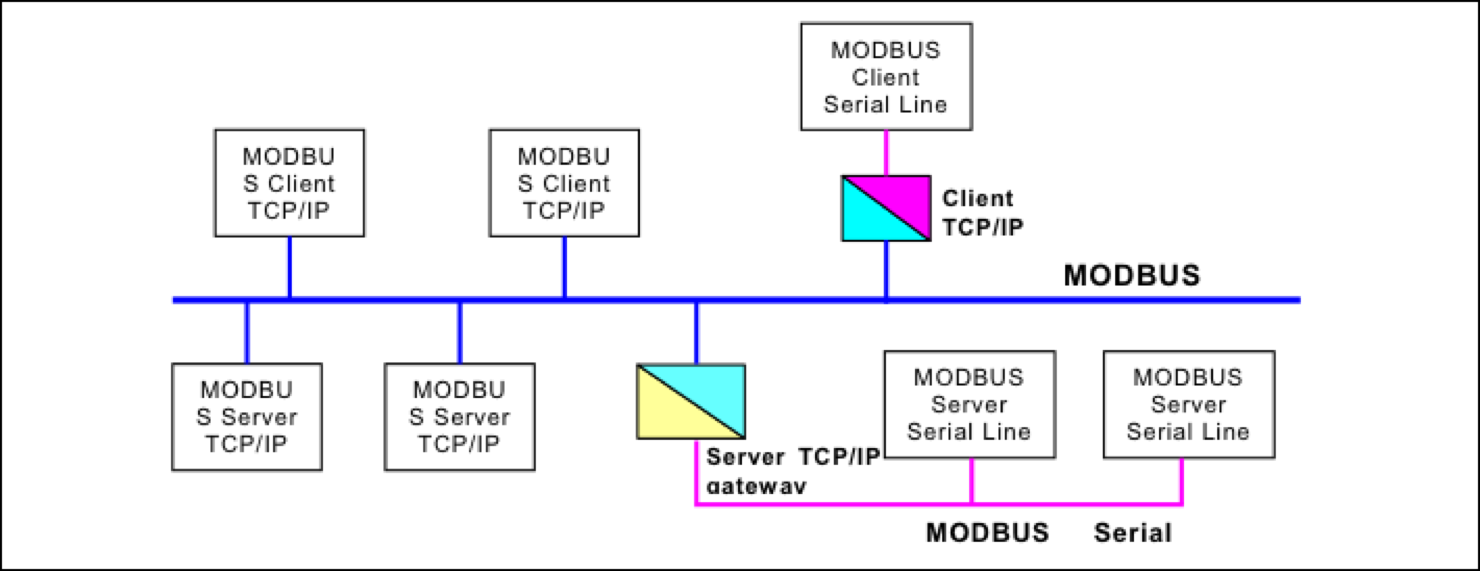
\includegraphics[width=\textwidth]{abbildungen/20160322_tcparchitektur}
\caption[Eine Modbus TCP/IP Kommunikationsarchitektur]{Eine Modbus TCP/IP Kommunikationsarchitektur, entnommen aus \cite[S.~4]{mod06tcp}}
\label{fig:tcparchiktektur}
\end{figure}

Das Modbus TCP Protokoll nutzt ein Master/Slave Buszugriffsverfahren, die Kommunikation hingegen ist anhand einer Client/Server Architektur aufgebaut. Dabei stellen lediglich die Clienten Anfragen, die vom angesprochenen Server beantwortet werden. Der Master schlüpft hierbei in die Rolle eines alleinigen Clienten.
Außerdem weicht die ADU leicht von der zuvor vorgestellten Version ab, wie in Abbildung \ref{fig:modbustcpframe} dargestellt. Die ADU enthält neben der PDU einen  \textit{Modbus Application Protocol Header} (MBAP), der sieben Bytes lang ist und die zusätzlichen Informationen zur Datenübertragung enthält. 
An erster Stelle im Header steht der \textit{Transaction Identifier}, der der Identifikation der Modbus TCP Telegramme dient. Darauf folgt der \textit{Protocol Identifier} der einen Wert von Null für das Modbus Protokoll annimmt. Das \textit{Length} Feld gibt durch einen Bytecount an, aus wie vielen Bytes das Telegramm besteht. Der Header wird durch den \textit{Unit Identifier}, analog zur Slave ID, abgeschlossen. Der Port 502 ist für Modbus Kommunikation reserviert, jedoch können auch andere Ports genutzt werden falls die Modbusgeräte eine Portkonfiguration unterstützen \cite[S.~4f.]{mod06tcp}

\begin{figure}
\centering
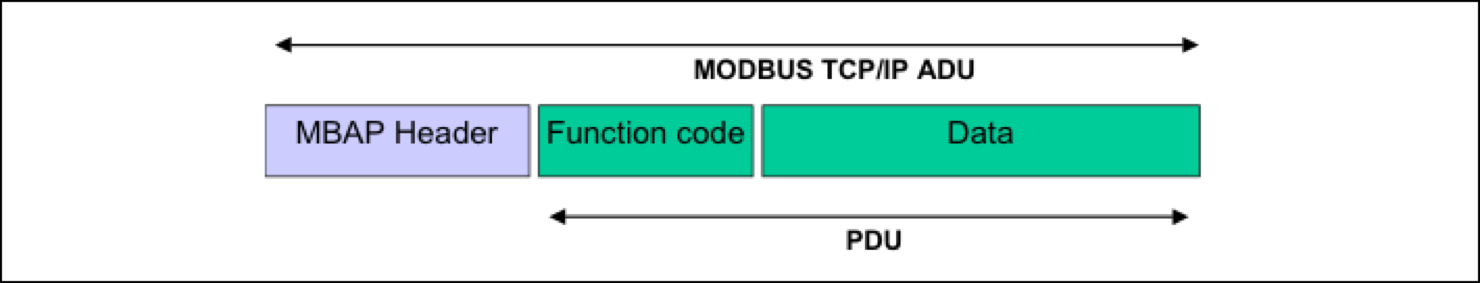
\includegraphics[width=\textwidth]{abbildungen/20160322_tcpframe}
\caption[Angepasster Rahmen für Telegramme nach dem Modbus TCP/IP Protokoll]{Angepasster Rahmen für Telegramme nach dem Modbus TCP/IP Protokoll, entnommen aus \cite[S.~4]{mod06tcp}}
\label{fig:modbustcpframe}
\end{figure}

Der Modbus Client initiiert den Informationsaustausch, indem er eine ADU erstellt und an den TCP Port 502 übermittelt. Die Modbus Server warten auf Anfragen über den TCP Port 502
\cite[S.~7f.]{mod06tcp}.
Das \textit{Transmission Control Protocol} (TCP) und das \textit{Internet Protokoll} (IP) übernehmen die Netzwerkaufgaben, entsprechend der Netzwerkschicht des OSI Modells. Dazu gehört die Bereitstellung eines Telegrammservices sowie das Einteilen der Daten in Transportdatenblöcke, wobei der MBAP Headers an jedes Paket angehängt wird \cite[S.~7ff.]{mod06tcp}.

Das Verbindungsmanagement wird vom TCP übernommen und ist sehr wichtig, da die Kommunikation verbindungsorientiert erfolgt.
Das Management kann durch ein externes Modul oder durch die Nutzeranwendung selbst erfolgen und umfasst den aktiven und passiven Auf- und Abbau von Verbindungen \cite[S.~11ff.]{mod06tcp}.
Zum Datenaustausch erfolgt der Aufbau einer Verbindung über das Ethernet IP Protokoll. Diese wird über die eindeutige IP Adresse des Gerätes im Netzwerk, die Port und \textit{Socket} Nummer hergestellt. Der Socket ist lediglich ein Endpunkt innerhalb eines Rechners, der einem Port eindeutig zugewiesen ist und über den die Kommunikation abläuft \cite[S.~15f.]{mod06tcp}.
Der interessierte Leser findet eine fundierte Einführung in die beiden Standards bei \cite{fu03}.

Der Leitfaden zur Implementierung des Modbus TCP Protokolls weist außerdem darauf hin, dass eine Verbindung nicht für jede einzelne Transaktion auf- und abgebaut werden muss, sondern endlos viele Modbus Transaktionen während einer Sitzung stattfinden können. Außerdem sollte die Anzahl an Verbindungen eines Server auf eine Minimum beschränkt werden \cite[S.~9f.]{mod06tcp}. Die physikalischen Schnittstellen werden durch das Ethernet als handelsüblicher Netzwerkanschluss spezifiziert.


\section{Technische Grundlagen zur Modellbildung}
\label{sec:grundlagenmodell}
In diesem Abschnitt werden die technischen Grundlagen zur Bildung eines mathematischen Modells eines Raumes in Kapitel \ref{chap:modellbildung} erläutert.

\subsection{Thermodynamische Systeme}

Für das Raummodell müssen Energieströme -- genauer betrachtet Wärmeströme -- untersucht werden. Um diese thermodynamischen Vorgänge mithilfe von Bilanzierungsgleichungen zu beschreiben, folgt zunächst ein kurze Einführung in die Thermodynamische Systembildung nach \cite[S.~11ff.]{ba12}.

\textit{Thermodynamische Systeme} werden durch den zu untersuchenden Raum abgegrenzt, der an den Grenzen von der Umgebung umgeben ist. Sie dienen dem Zweck der Bilanzierung von Massen- und Energieströmen. Die begrenzenden Flächen können gedanklicher, physischer oder beider Art zugleich sein, wichtig ist das die Systemgrenzen eindeutig festgelegt sind \cite[S.~11]{ba12}.

Anhand der Eigenschaften von den Systemgrenzen lassen sich die thermodynamischen Systeme weiter differenzieren.
Solche Systeme, deren Grenzen undurchlässig für Materie sind, werden als \textit{geschlossene Systeme} bezeichnet und werden durch eine konstante Stoffmenge innerhalb des Systems gekennzeichnet. Die Grenzen eines geschlossenen Systems sind meistens räumlich anhand eines fixen Volumens definiert, können aber auch beweglich sein, wie beispielsweise das Volumen einer vorgegebenen Stoffmenge unabhängig von dessen räumlicher Ausdehnung \cite[S.~12]{ba12}.

Sind die Grenzen von thermodynamischen Systemen für Materie durchlässig, werden diese als \textit{offene Systeme} bezeichnet. In der Regel werden diese von Stoffströmen durchflossen und durch räumlich festgelegte Grenzen beschrieben. Diese werden in der Literatur auch als \textit{Kontrollraum} oder \textit{Kontrollvolumen} bezeichnet \cite[S.~12]{ba12}.

Ein \textit{abgeschlossenes System} umfasst in der Regel mehrere Systeme oder ein einzelnes System und dessen Umgebung, so dass es zwischen den Grenzen des abgeschlossenen Systems und seiner Umgebung keine Wechselwirkungen gibt. Die Systemgrenzen werden so gelegt, dass über sie hinweg keine \acrlong{bzw} keine relevanten\footnote{\textit{Relevant} im Sinne von kaum messbarer Fluss und nicht messbare Auswirkung auf das System.} Flüsse von Materie und Energie stattfinden \cite[S.~13]{ba12}.

Nach der Abgrenzung folgt die Beschreibung von thermodynamischen Systemen und dessen \textit{Eigenschaften}. Diese erfolgt durch \textit{Variablen} und \textit{physikalische Größen} die ein System kennzeichnen. Die Variablen, welche den \textit{Zustand} eines Systems bestimmen, werden diese als \textit{Zustandsgrößen} bezeichnet \cite[S.~13]{ba12}. Im Rahmen der Modellbildung in Kapitel \ref{chap:modellbildung} ist es ausreichend die Vorgänge und Effekte auf systemischer Ebene zu betrachten, wodurch sich Modelle mit wenigen Variablen und physikalischen Größen beschreiben lassen.

Die Variablen lassen sich in \textit{äußere Größen}, welche den mechanischen Zustand eines Systems beschreiben\footnote{Zum Beispiel die Koordinaten im Raum oder die relative Geschwindigkeit zum Beobachter)}, und \textit{innere Größen} gliedern, welche den thermodynamischen Zustand, also die Eigenschaften der Materie innerhalb der Systemgrenzen, beschreiben\cite[S.13~f.]{ba12}.

Innerhalb der Grenzen eines thermodynamischen Systems, und damit implizit auch für das Raummodell wird \textit{Homogenität} angenommen. Dies bedeutet, dass die physikalischen Eigenschaften, wie \acrlong{zb} Temperatur und Druck, sowie die chemische Zusammensetzung an jeder Stelle innerhalb des Systems die gleiche Ausprägung besitzt \cite[S.15]{ba12}.

Da wir im Rahmen der Modellbildung Zustände betrachten, müssen auch deren Änderungen genauer untersucht werden. Die \textit{Zustandsänderungen} eines Systems werden durch Änderungen von Energie oder Materie über dessen Grenzen hinweg bedingt und finden meist im Austausch der Umgebung statt. Während einer solchen Änderung des Systemzustands wird ein Prozess durchlaufen, der eine zeitliche Abfolge von Ereignissen ist. Eine Änderung des Zustandes eines Systems mit einer gleichen Wirkung, kann also durch verschiedene Prozesse bewirkt werden. Daher beschreibt ein \textit{Prozess} nicht nur die Veränderung des Zustands, sondern viel mehr die Beziehungen zwischen einem System und seiner Umgebung \cite[S.21~f.]{ba12}.

Ein Prozess kann aber auch innerhalb eines Systems stattfinden, dass heißt ohne äußere Einwirkungen. Dies geschieht zum Beispiel durch das Aufheben innerer Hemmungen oder dem Wegfall von äußeren Zwängen. Diese Prozesse laufen in abgeschlossenen Systemen meist von selbst ab und streben einen ausgeglichenen, also homogenen, Endzustand an. \textit{Ausgleichsprozesse} dienen dazu, einen \textit{Gleichgewichtszustand} zu erreichen und repräsentieren Wechselwirkungen zwischen verschiedenen Teilen eines abgeschlossenen Systems. Dabei gleichen sich die Zustandsgrößen von einzelnen Subsystemen wie zum Beispiel der Druck oder die Temperatur einander an. Der Gleichgewichtszustand wird also durch die Zustände in den einzelnen Subsystemen bestimmt und ist dadurch charakterisiert, dass ein System diesen Zustand nicht von sich aus, sondern nur durch äußere Eingriffe verlässt, beispielsweise durch eine Veränderungen in der Umgebung. Die Erfahrung lehrt, dass ein System einem Gleichgewichtszustand entgegen strebt, wenn es sich selbst überlassen wird \cite[S.22~f.]{ba12}.

\subsection{Erster Hauptsatz der Thermodynamik}

Der erste Hauptsatz der Thermodynamik wird zunöchst als allgemeiner Energieerhaltungssatz formuliert und anschließend angewandt, um eine Energiebilanzgleichung für geschlossene thermodynamische Systeme zu erhalten.

Der erste Hauptsatz der Thermodynamik erweitert den mechanischen Energieerhaltungssatz um die Energieformen Wärme und innere Energie. Er handelt ganz allgemein vom Prinzip der Energieerhaltung und  dient er der Bilanzierung von Systemen \cite[S.~43]{ba12}.

Die Gesamtenergie eines Systems \gls{e} setzt sich zusammen aus der potenziellen \gls{epot} und kinetischen Energie \gls{ekin} wie in der Mechanik und wird durch die innere Energie \gls{u} ergänzt \cite[S.~49]{ba12}:

\begin{equation}
\label{eq:energie}
E := E_{pot} + E_{kin} + U
\end{equation}

Im weiteren Verlauf der Arbeit werden nur ortsfeste Systeme betrachtet, die sich dadurch auszeichnen, dass deren potenzielle Energie  \gls{epot} in etwa konstant ist. Weiterhin erfahren sie im betrachteten Intertialsystem Erde auch nur sehr kleine Änderungen in ihrer Geschwindigkeit, weshalb auch die kinetische Energie \gls{ekin} in etwa konstant ist.  Da die Änderungen der mechanischen Energien in Bezug auf die Änderung der inneren Energie sehr klein sind, werden im Folgenden nicht weiter betrachtet und die Gesamtenergie eines Systems \gls{e} wird vereinfacht und lediglich aus der inneren Energie bestehend angenommen.

Die innere Energie hängt von der spezifischen Wärmekapazität \gls{cp}, der Masse eines Systems \gls{msys} und der Temperatur \gls{t} \acrlong{bzw} \gls{T} ab \cite[S.~54]{ba12}:

\begin{equation}
\label{eq:innereenergie}
U := m*c_p*T=m*c_p*t+u_0,~mit~t=T-T_0
\end{equation}

Nach dem Prinzip der Energieerhaltung, kann die Energie eines Systems weder erzeugt noch vernichtet, sondern lediglich durch den Energietransport über dessen Grenzen hinweg verändert werden. Daraus ergeben sich folgende qualitative Formen des Energietransports \cite[S.~48f.]{ba12}:

\begin{itemize}
	\item Die Arbeit \gls{w}, die entweder von oder an einem System verrichtet wird, in differentieller Form die Leistung \gls{p}.
	\item Die Wärme \gls{q}, die entweder in das System hinein- oder herausfließt, in differentieller Form der Wärmestrom \gls{qdot}.
	\item Der Transport von Materie, also das Einbringen oder Wegnehmen von Masse \gls{m} eines System, in differentieller Form die Materialflüsse \gls{mdot}.
\end{itemize}

Mit der zuvor getroffenen Annahme, dass die innere Energie der des Systems entspricht, und unter Beachtung der Vorzeichenkonvention, welche besagt dass zugeführte Energie positiv und abgeführte Energie negativ zu bewerten ist, lassen sich die Änderungen der Energie eines Systems mit der folgenden Gleichung quantitativ beschreiben \cite[S.~54]{ba12}:

\begin{equation}
\label{eq:hauptsatz}
\begin{split}
\Delta U & = Q + W + m_{in}*c_{p}*T_{in}-m_{out}*c_{p}*T_{out} \\ ~& \mathrm{beziehungsweise~in~differentieller~Form}\\
\frac{dU}{dt}=\dot{U} & =\dot{Q}+P+\sum\dot{m}_{in}*c_{p}*T_{in}-\sum\dot{m}_{out}*c_{p}*T_{out}
\end{split}
\end{equation}


\subsection{Wärmeübertragung}

Wie zuvor erwähnt haben Wärmeströme eine zentrale Bedeutung bei der Modellbildung, weshalb ein genauere Betrachtung folgt.

Die Definition von Wärmeübertragung ist nach \cite[S.~1]{bo14} \Gun [...] der Transfer der Energieform Wärme aufgrund einer Temperaturdifferenz. \Gun .
Die Wärmeübertragung kann nach \textit{Nußelt}\footnote{Beschrieben in seinem Aufsatz \Gun Das Grundgesetz des Wärmeüberganges\Gob , 1915.} grundsätzlich durch zwei verschiedene Arten stattfinden \cite[S.~3f.]{bo14}:

\begin{itemize}
	\item Wärmeübertragung durch Strahlung, bei der die Übertragung von Wärme ohne stofflichen Träger, lediglich durch elektromagnetische Wellen zwischen Oberflächen erfolgt. Weil diese Art der Wärmeübertragung keine Relevanz für die weiteren Betrachtungen hat wird er interessierte Leser für eine fundierte Einführung an \cite{bo14} verwiesen. 
	\item  Wärmeübertragung durch Wärmeleitung, die sich wiederum in die Wärmeübertragung zwischen ruhenden Stoffen, und die Konvektion, die eine Wärmeübertragung zwischen einem ruhenden und einem strömenden Fluid beschreibt, aufteilen lässt. 
\end{itemize}

Die übertragene Wärmemenge ist bei der reinen Wärmeleitung lediglich von den Stoffeigenschaften und der Temperaturdifferenz abhängig, bei der Konvektion hingegen hängt sie von der Strömung der Fluide ab, unabhängig davon ob erzwungene oder freie Konvektion. Die Konvektion ist ein Effekt, der zusätzlich zur reinen Wärmeleitung auftritt ebenfalls nicht relevant für den weiteren Verlauf ist und detaillreich von \cite{bo14} beschrieben wird.
Erfolgt der Wärmetransport stationär, dass heißt von äußeren Anregungen bedingt und unabhängig von der Zeit, lässt er sich qualitativ einfach als konstanter Wärmestrom \gls{qdot} beschreiben. Er gibt, an wie viel Wärme pro Sekunde übertragen werden \cite[S.~5ff.]{bo14}. 
Der Wärmestrom ist wie zuvor bereits erwähnt von den Stoffeigenschaften abhängig, welche von der Wärmedurchgangszahl \gls{uwert}\footnote{Der U-Wert wurde bis zu der Umstellung auf die europäischen Prüfnormen 2003 als k-Wert bezeichnet und ist unter dieser Bezeichnung noch häufig in der Literatur zu finden \cite[S.1~f.]{sa04}} und der Austauschoberfläche \gls{A}, an welcher der Wärmeaustausch stattfindet. Typische U-Werte für verschiedene Materialien und Komponenten finden in der einschlägigen Literatur und beziehen sich bei der Übertragung durch eine Wand im europäischen Raum auf die Außenfläche \cite[S.~28]{bo14}. Damit lässt sich der Wärmestrom unter Berücksichtigung der Abhängigkeiten durch die kinetische Kopplungsgleichung quantifizieren \cite[S.~6f.]{bo14}:

\begin{equation}
\label{eq:qdot}
\dot{Q} := u*A*(t_{1}-t_{2})
\end{equation}

Unterschiedliche geometrische Ausprägungen, wie zum Beispiel ein Wärmeaustausch durch eine Wand oder ein Rohr hindurch, finden damit implizit bei der Austauschoberfläche Berücksichtigung.